%%%%%%%%%%%%%%%%%%%%%%%%%%%%%%%%%%%%%%%%%
% Short Sectioned Assignment LaTeX Template Version 1.0 (5/5/12)
% This template has been downloaded from: http://www.LaTeXTemplates.com
% Original author:  Frits Wenneker (http://www.howtotex.com)
% License: CC BY-NC-SA 3.0 (http://creativecommons.org/licenses/by-nc-sa/3.0/)
%%%%%%%%%%%%%%%%%%%%%%%%%%%%%%%%%%%%%%%%%

%----------------------------------------------------------------------------------------
%	PACKAGES AND OTHER DOCUMENT CONFIGURATIONS
%----------------------------------------------------------------------------------------

\documentclass[paper=a4, fontsize=11pt]{scrartcl} % A4 paper and 11pt font size

% ---- Entrada y salida de texto -----

\usepackage[T1]{fontenc} % Use 8-bit encoding that has 256 glyphs
\usepackage[utf8]{inputenc}
%\usepackage{fourier} % Use the Adobe Utopia font for the document - comment this line to return to the LaTeX default

% ---- Idioma --------

\usepackage[spanish, es-tabla]{babel} % Selecciona el español para palabras introducidas automáticamente, p.ej. "septiembre" en la fecha y especifica que se use la palabra Tabla en vez de Cuadro

% ---- Otros paquetes ----

\usepackage[hidelinks]{hyperref} % Estilo para los enlaces
\hypersetup{
  colorlinks   = true, %Colours links instead of ugly boxes
  urlcolor     = blue, %Colour for external hyperlinks
  linkcolor    = black, %Colour of internal links
  citecolor   = blue %Colour of citations
}
\usepackage{url} % ,href} %para incluir URLs e hipervínculos dentro del texto (aunque hay que instalar href)
\usepackage{amsmath,amsfonts,amsthm} % Math packages
%\usepackage{graphics,graphicx, floatrow} %para incluir imágenes y notas en las imágenes
\usepackage{graphics,graphicx, float} %para incluir imágenes y colocarlas
\usepackage{eurosym}

% Para hacer tablas comlejas
%\usepackage{multirow}
%\usepackage{threeparttable}

%\usepackage{sectsty} % Allows customizing section commands
%\allsectionsfont{\centering \normalfont\scshape} % Make all sections centered, the default font and small caps

\usepackage{fancyhdr} % Custom headers and footers
\pagestyle{fancyplain} % Makes all pages in the document conform to the custom headers and footers
\fancyhead{} % No page header - if you want one, create it in the same way as the footers below
\fancyfoot[L]{} % Empty left footer
\fancyfoot[C]{} % Empty center footer
\fancyfoot[R]{\thepage} % Page numbering for right footer
\renewcommand{\headrulewidth}{0pt} % Remove header underlines
\renewcommand{\footrulewidth}{0pt} % Remove footer underlines
\setlength{\headheight}{13.6pt} % Customize the height of the header

\numberwithin{equation}{section} % Number equations within sections (i.e. 1.1, 1.2, 2.1, 2.2 instead of 1, 2, 3, 4)
\numberwithin{figure}{section} % Number figures within sections (i.e. 1.1, 1.2, 2.1, 2.2 instead of 1, 2, 3, 4)
\numberwithin{table}{section} % Number tables within sections (i.e. 1.1, 1.2, 2.1, 2.2 instead of 1, 2, 3, 4)

\setlength\parindent{0pt} % Removes all indentation from paragraphs - comment this line for an assignment with lots of text

\newcommand{\horrule}[1]{\rule{\linewidth}{#1}} % Create horizontal rule command with 1 argument of height


%----------------------------------------------------------------------------------------
%	TÍTULO Y DATOS DEL ALUMNO
%----------------------------------------------------------------------------------------

\title{	
\normalfont \normalsize 
\textsc{\textbf{Ingeniería de Servidores (2016-2017)} \\ Grado en Ingeniería Informática \\ Universidad de Granada} \\ [25pt] % Your university, school and/or department name(s)
\horrule{0.5pt} \\[0.4cm] % Thin top horizontal rule
\huge Memoria Práctica 4 \\ % The assignment title
\horrule{2pt} \\[0.5cm] % Thick bottom horizontal rule
}

\author{Elena María Gómez Ríos} % Nombre y apellidos

\date{\normalsize\today} % Incluye la fecha actual

%----------------------------------------------------------------------------------------
% DOCUMENTO
%----------------------------------------------------------------------------------------

\begin{document}

\maketitle % Muestra el Título

\newpage %inserta un salto de página

\tableofcontents % para generar el índice de contenidos

\listoffigures

\listoftables

\newpage

%\textbf{NOTA: en caso de problema al compilar, compruebe que tiene el paquete: texlive-babel-spanish.noarch }  \\
 


\newpage

%----------------------------------------------------------------------------------------
%	Cuestión 1
%----------------------------------------------------------------------------------------

\section{Cuestión 1:}

\subsection{a) ¿Seleccione, instale y ejecute uno, comente los resultados. Atención: no es lo mismo un benchmark que una suite, instale un benchmark.}

Para instalar Phoronix Suite en CentOS \cite{phoronix} se utiliza el comando  \texttt{yum install \\ phoronix-test-suite} (figura \ref{fig:ejercicio1_1}). Con el comando \texttt{phoronix-test-suite list-tests} se obtiene una lista de los benchmarks disponibles (figura \ref{fig:ejercicio1_2}). Para intalar un benchmark de la lista se utiliza el comando \texttt{phoronix-test-suite install <test>} (figura \ref{fig:ejercicio1_3}).

La documentación utilizada para los comandos de phoronix ha sido \cite{phoroniComandos}, aunque podemos obtener la misma información con \texttt{man phoronix-test-suite}.\\

Podemos iniciar el cliente web con el comando \texttt{phoronix-test-suite gui} (figura \ref{fig:ejercicio1_4}), el cual abrirá una nueva ventana como se muestra en la figura \ref{fig:ejercicio1_5} en la que aparece la monitorización de nuestro sistema. Desde aquí también podemos listar los test disponibles (figura \ref{fig:ejercicio1_6}) e instalarlos. En la pestaña de ``Installed Tests'' podemos ver los benchmarks ya instalados, en mi caso, como se muestra en la figura \ref{fig:ejercicio1_7}, aparece el ``Blender'' que es el benchmark que he instalado anteriormente.\\

Ejecutar el bechmark desde la GUI es muy sencillo, simplemente debemos pulsar sobre el bechmark que queremos ejecutar y nos saldrá una pantalla como la de la figura \ref{fig:ejercicio1_8}, si el benchmark no está instalado se instalará previamente. Mientras que se ejecuta el benchmark se muestra la siguiente pantalla de información, figura \ref{fig:ejercicio1_9}, donde informa del tiempo aproximado que va a tardar en completarse.\\

Debido a que mi máquina virtual no es capaz de finalizar el benchmark de Blender, he decidido cancelar la ejecución tras unos 46 minutos (figura \ref{fig:ejercicio1_10}) y probar con otro que requiera menos requisitos y tarde menos en finalizar la ejecución, como por ejemplo ``GLmark2'' (figura \ref{fig:ejercicio1_11} y \ref{fig:ejercicio1_12}).\\

Una vez finalizado el benchmark de ``GLmark2'', como se muestra en la figura \ref{fig:ejercicio1_13}, accedemos a los resultados donde podemos ver un listado de las especificaciones de nuestro sistema y una puntuación del test realizado(figuras \ref{fig:ejercicio1_14} y \ref{fig:ejercicio1_15}).



\begin{figure}[H] 
	\centering
	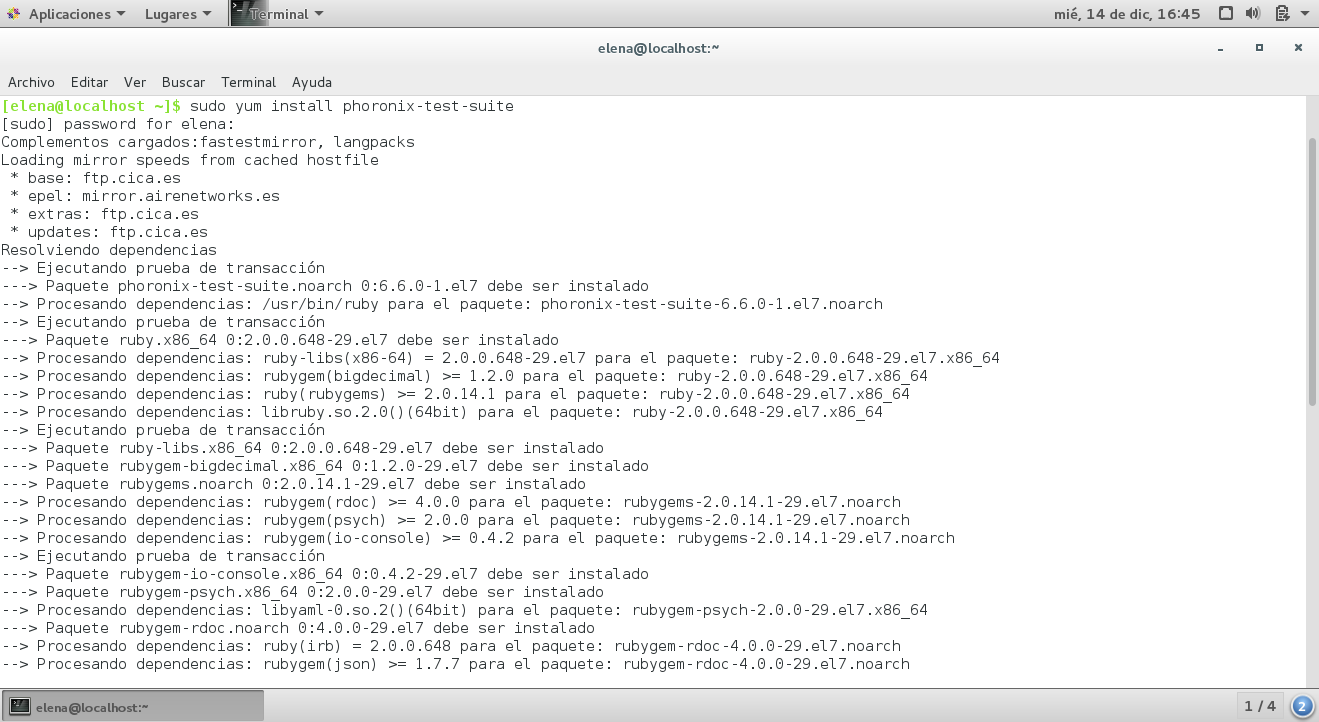
\includegraphics[width=14.7cm]{./img/ejercicio1_1.png} 	
	\caption{CentOS, instalación de Phoronix Suite.} \label{fig:ejercicio1_1}
\end{figure}

\begin{figure}[H] 
	\centering
	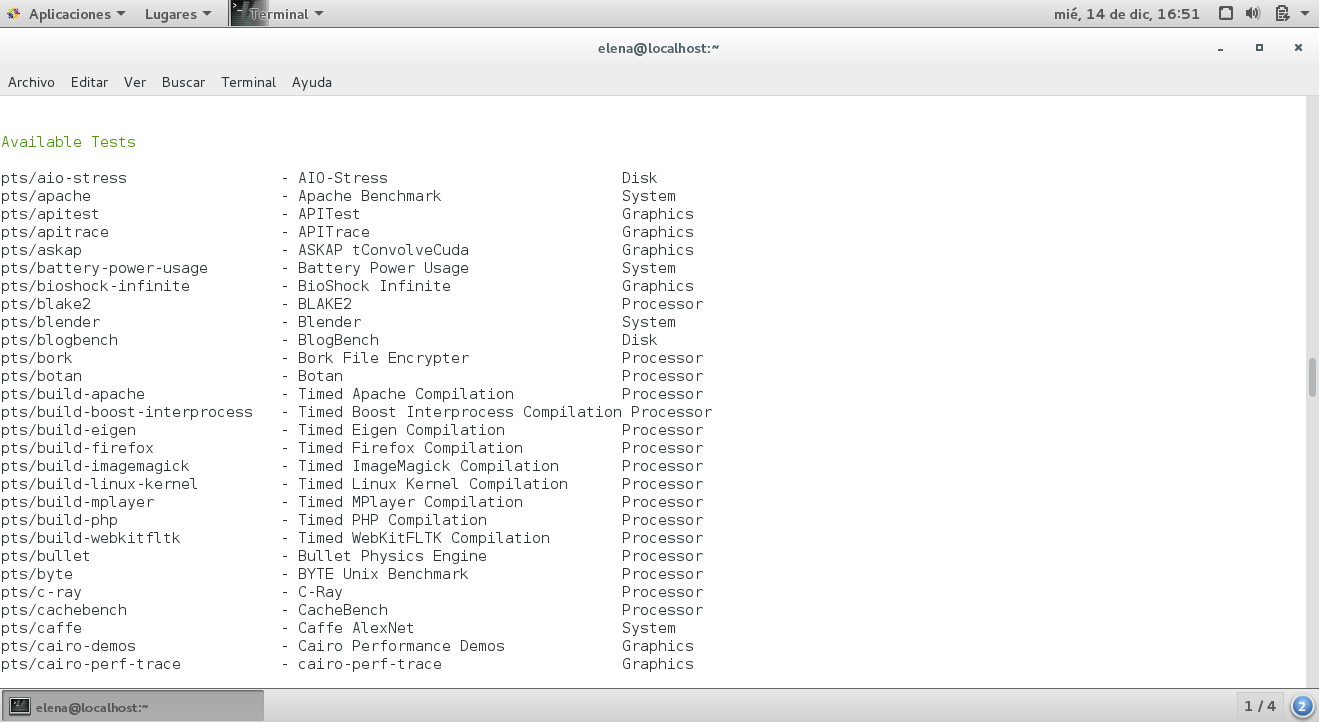
\includegraphics[width=14.7cm]{./img/ejercicio1_2.png} 	
	\caption{CentOS, listado de benchmarks.} \label{fig:ejercicio1_2}
\end{figure}

\begin{figure}[H] 
	\centering
	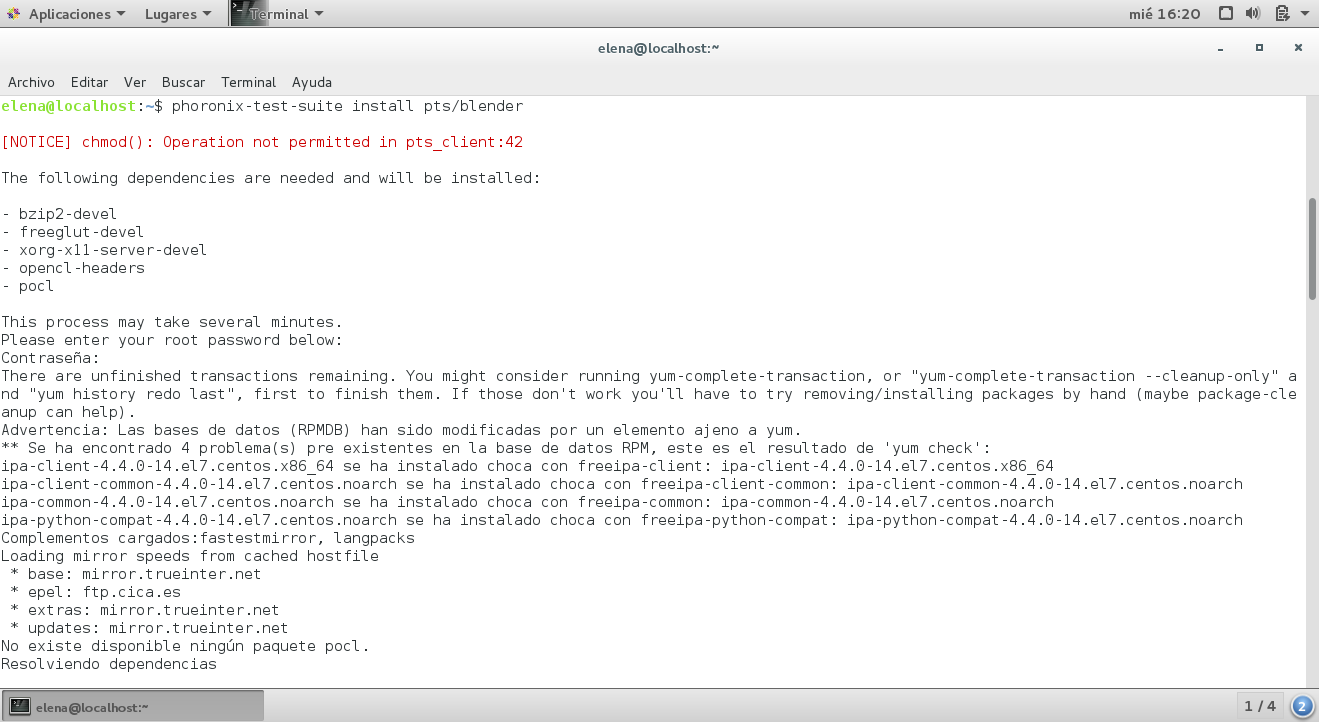
\includegraphics[width=14.7cm]{./img/ejercicio1_3.png} 	
	\caption{CentOS, instalación del benchmark Blender.} \label{fig:ejercicio1_3}
\end{figure}

\begin{figure}[H] 
	\centering
	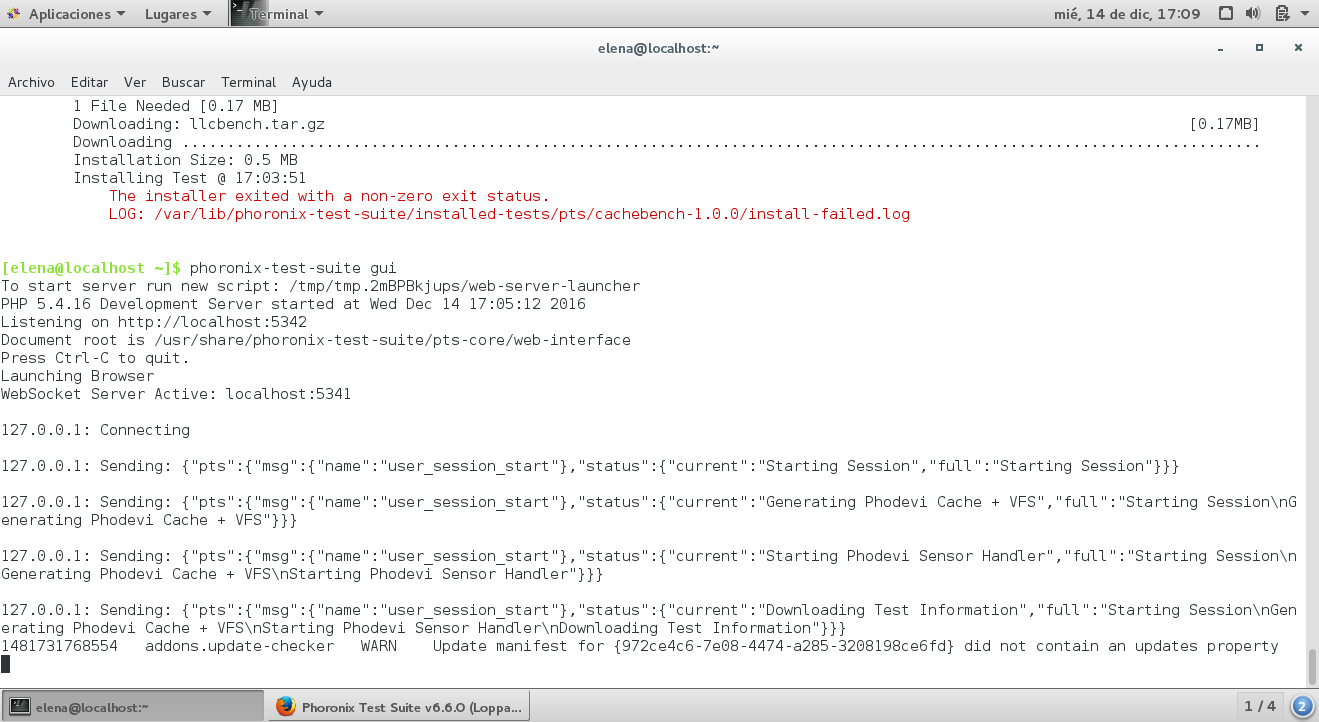
\includegraphics[width=14.7cm]{./img/ejercicio1_4.png} 	
	\caption{CentOS, Phoronix Suite GUI.} \label{fig:ejercicio1_4}
\end{figure}

\begin{figure}[H] 
	\centering
	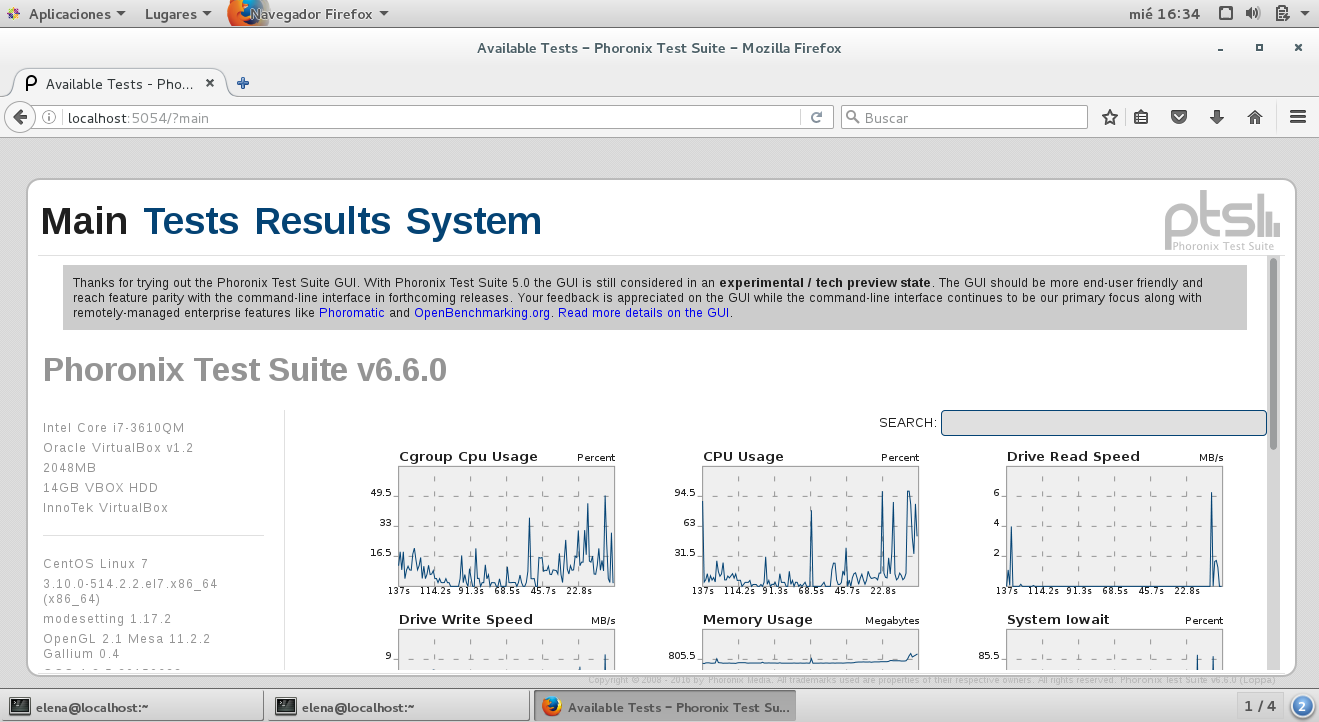
\includegraphics[width=14.7cm]{./img/ejercicio1_5.png} 	
	\caption{CentOS, Phoronix Suite GUI web.} \label{fig:ejercicio1_5}
\end{figure}

\begin{figure}[H] 
	\centering
	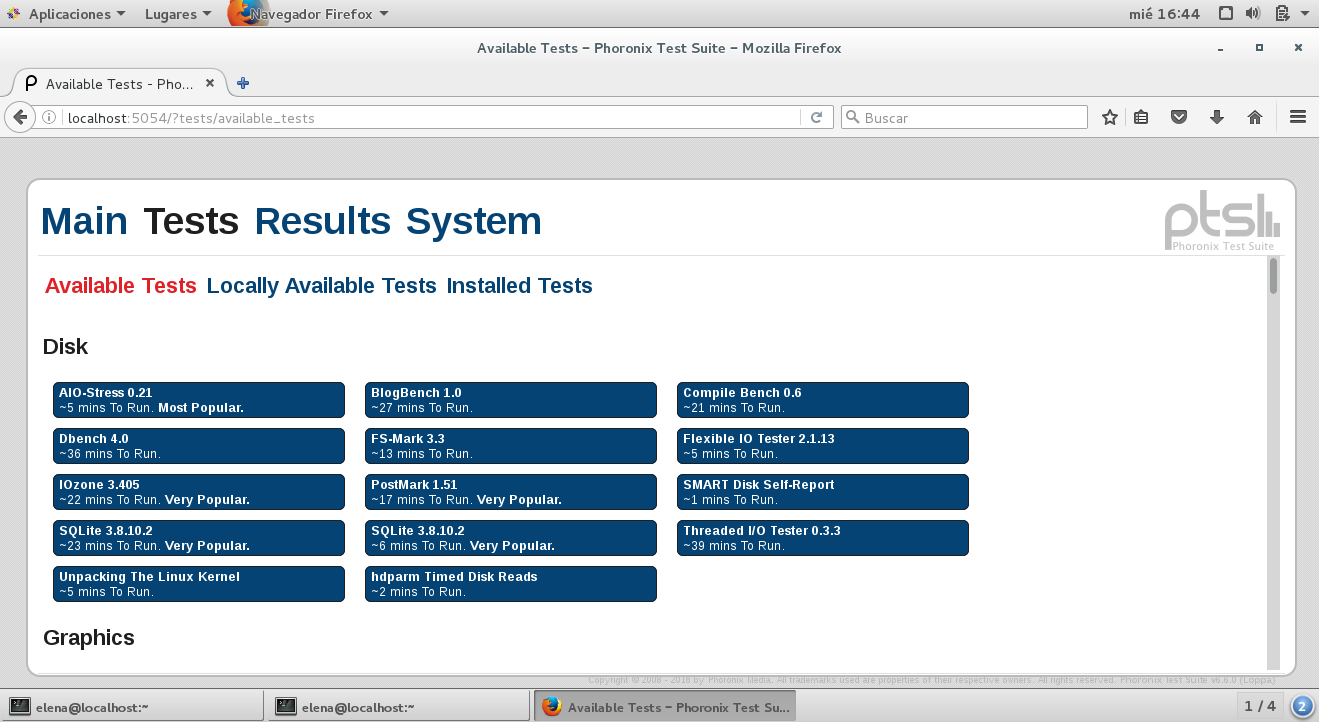
\includegraphics[width=14.7cm]{./img/ejercicio1_6.png} 	
	\caption{CentOS, Phoronix Suite, listado de benchmarks.} \label{fig:ejercicio1_6}
\end{figure}

\begin{figure}[H] 
	\centering
	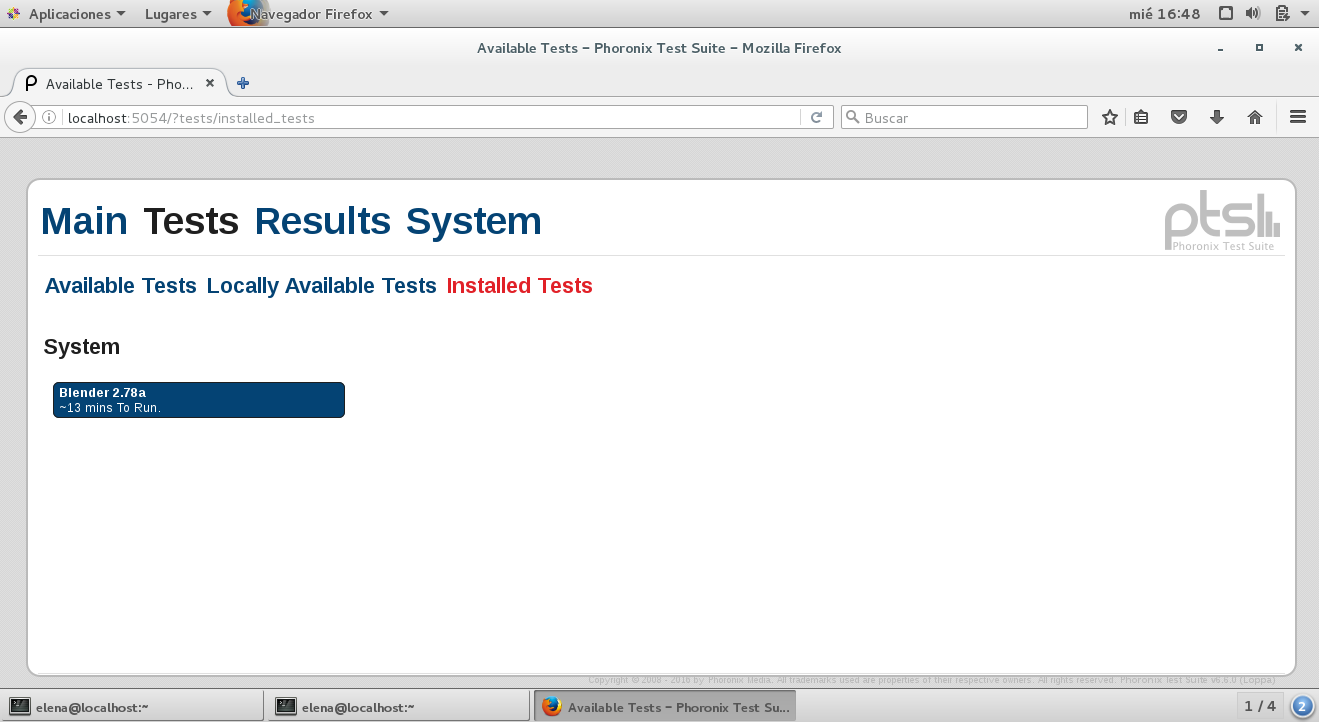
\includegraphics[width=14.7cm]{./img/ejercicio1_7.png} 	
	\caption{CentOS, Phoronix Suite, listado de benchmarks instalados.} \label{fig:ejercicio1_7}
\end{figure}

\begin{figure}[H] 
	\centering
	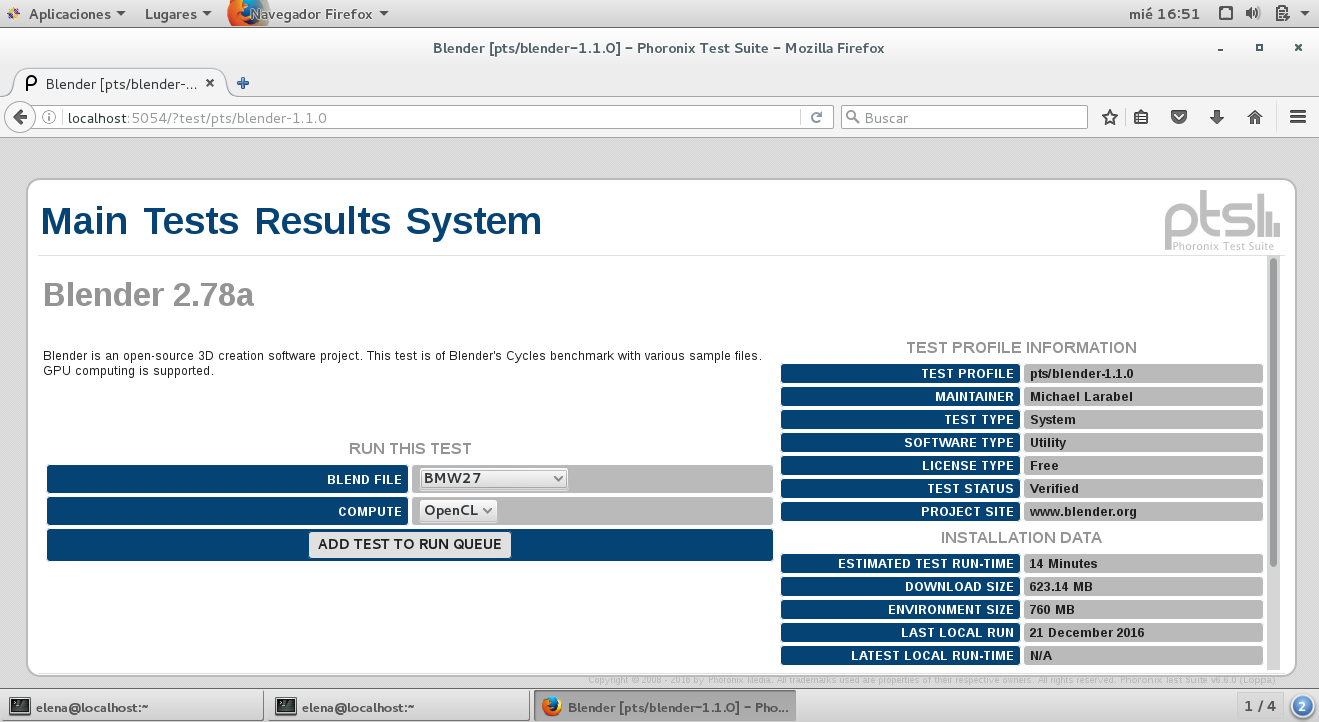
\includegraphics[width=14.7cm]{./img/ejercicio1_8.png} 	
	\caption{CentOS, Phoronix Suite, ejecución de benchmarks.} \label{fig:ejercicio1_8}
\end{figure}

\begin{figure}[H] 
	\centering
	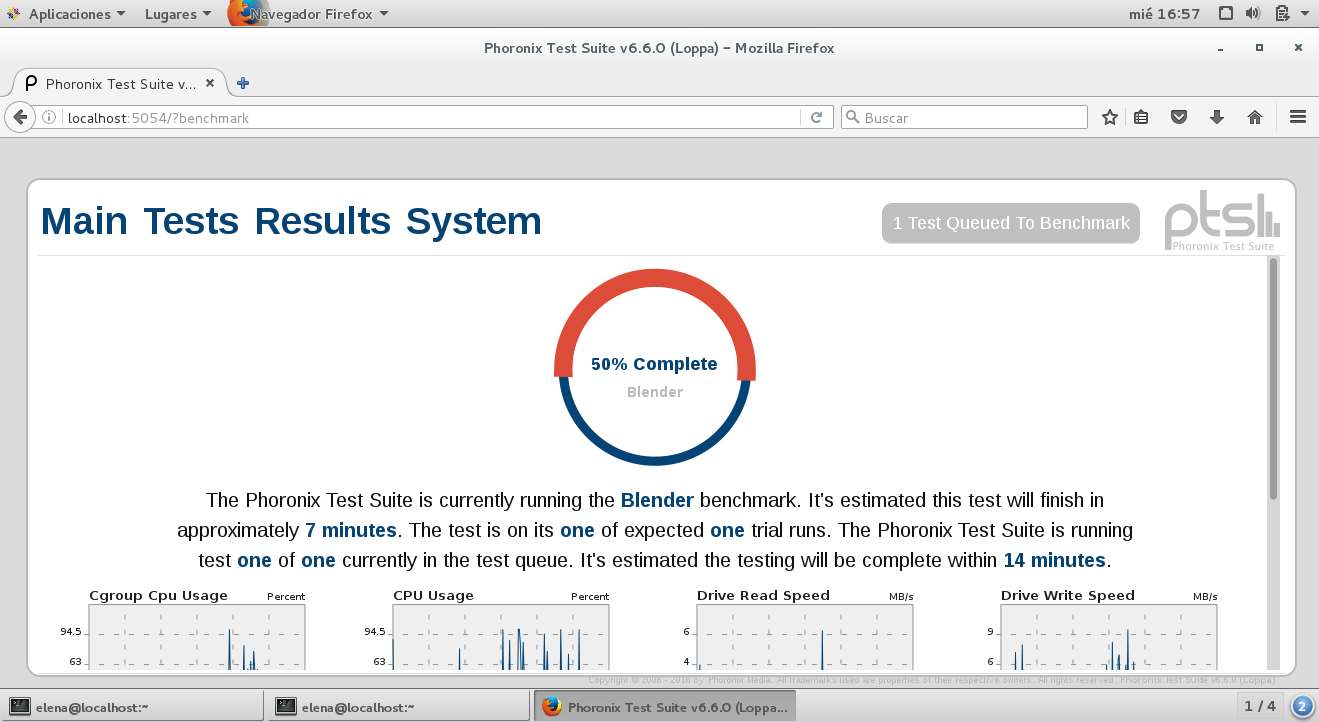
\includegraphics[width=14.7cm]{./img/ejercicio1_9.png} 	
	\caption{CentOS, Phoronix Suite, ejecución de benchmarks.} \label{fig:ejercicio1_9}
\end{figure}

\begin{figure}[H] 
	\centering
	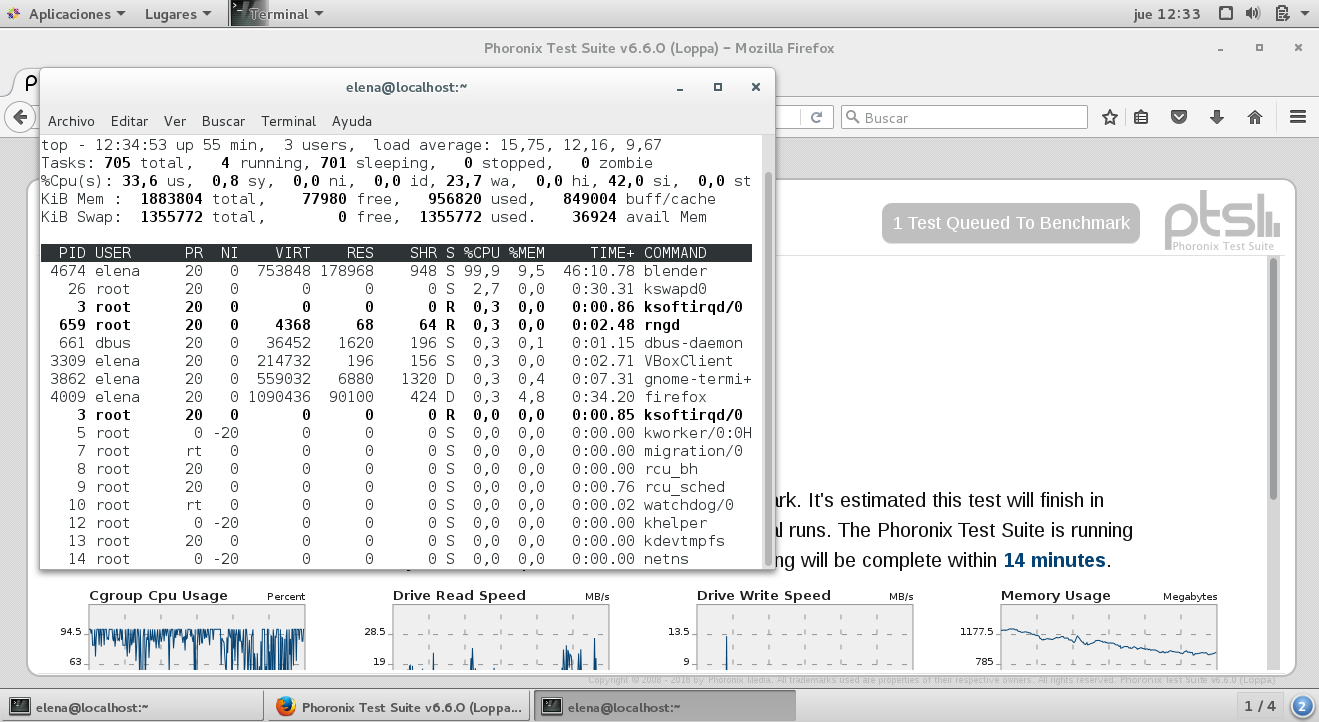
\includegraphics[width=14.7cm]{./img/ejercicio1_10.png} 	
	\caption{CentOS, Phoronix Suite, problemas con benchmark Blender.} \label{fig:ejercicio1_10}
\end{figure}

\begin{figure}[H] 
	\centering
	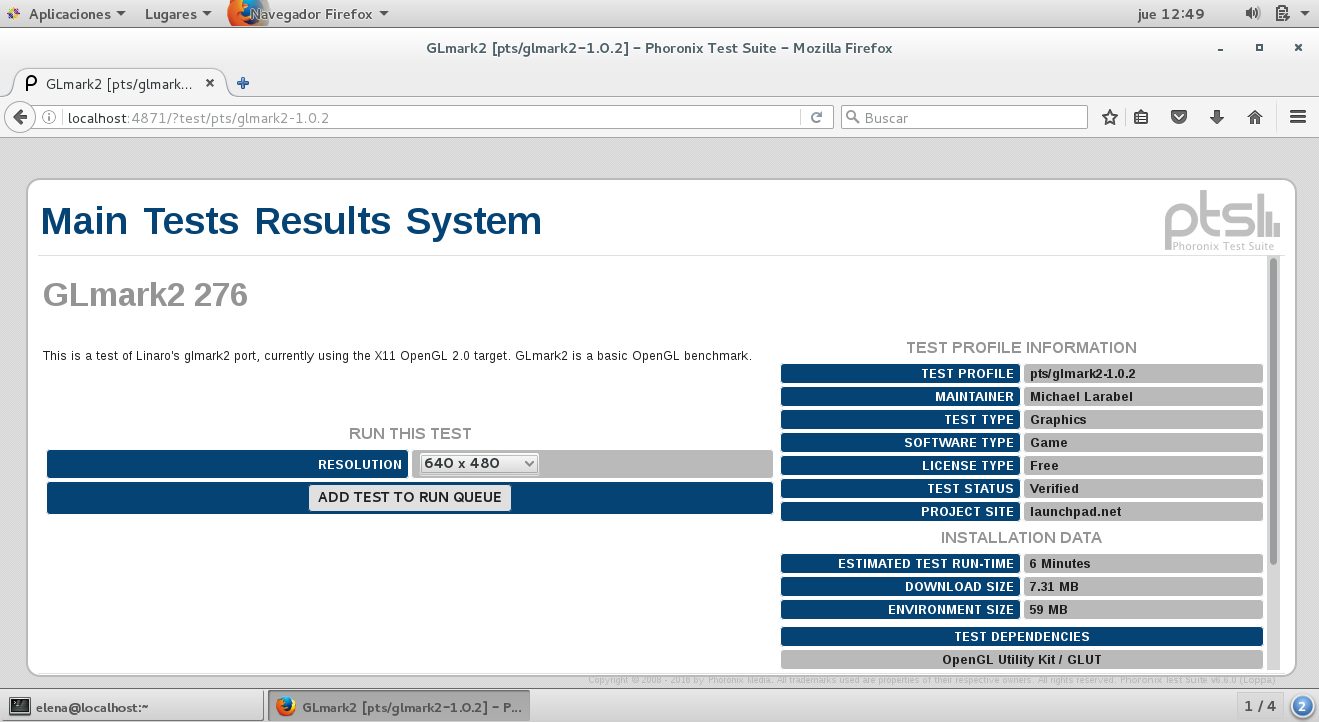
\includegraphics[width=14.7cm]{./img/ejercicio1_11.png} 	
	\caption{CentOS, Phoronix Suite, ejecución de benchmark GLmark2.} \label{fig:ejercicio1_11}
\end{figure}

\begin{figure}[H] 
	\centering
	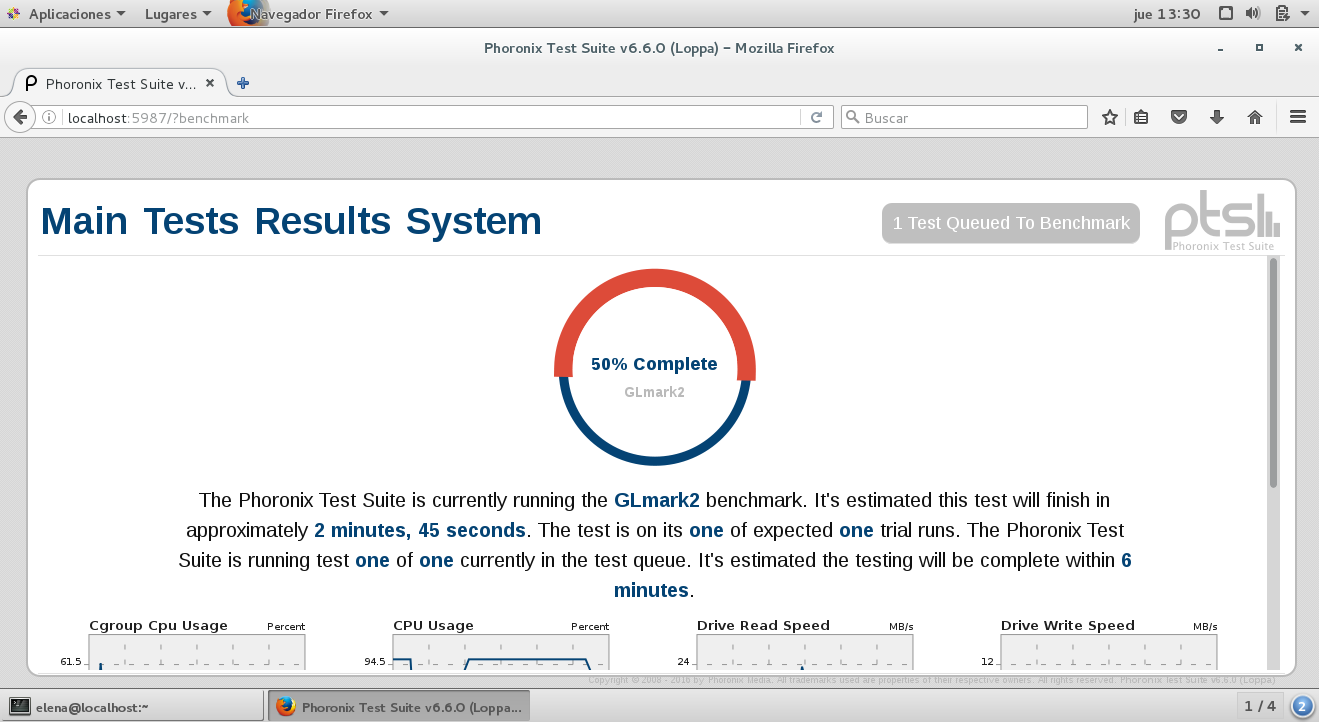
\includegraphics[width=14.7cm]{./img/ejercicio1_12.png} 	
	\caption{CentOS, Phoronix Suite, ejecución de benchmark GLmark2.} \label{fig:ejercicio1_12}
\end{figure}

\begin{figure}[H] 
	\centering
	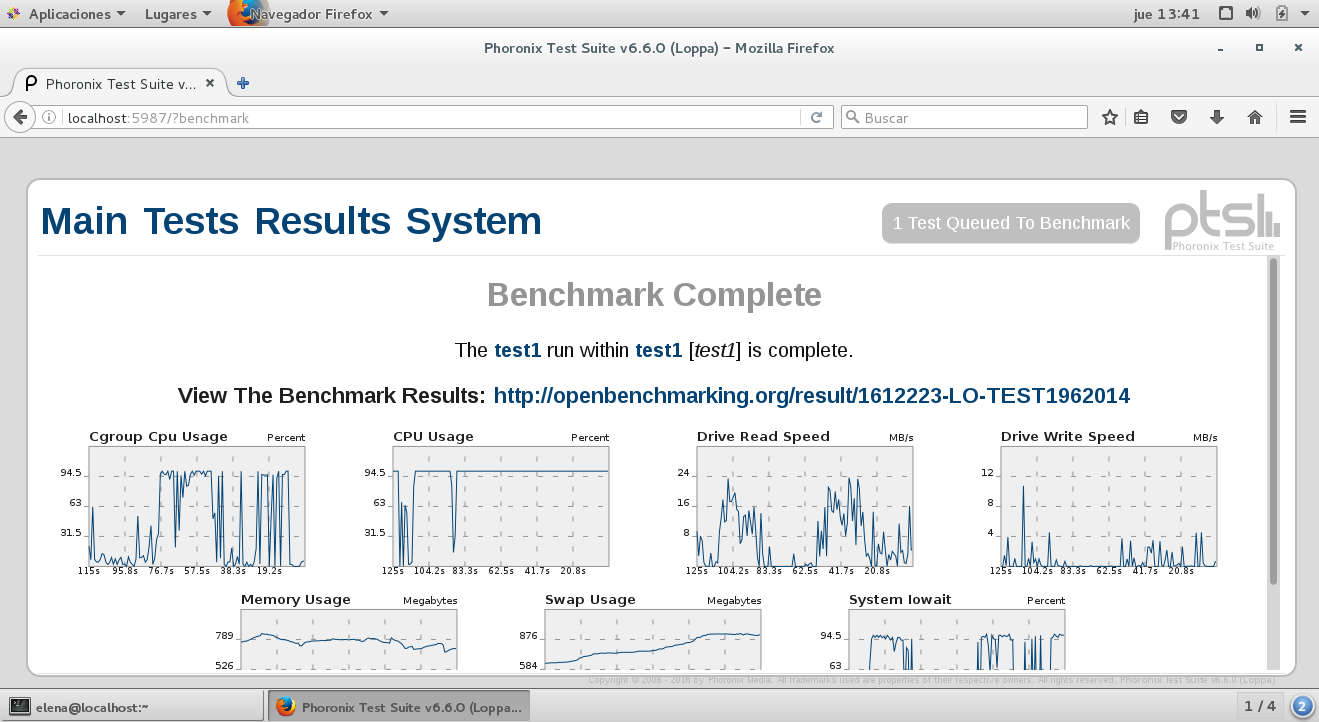
\includegraphics[width=14.7cm]{./img/ejercicio1_13.png} 	
	\caption{CentOS, Phoronix Suite, benchmark GLmark2 finalizado.} \label{fig:ejercicio1_13}
\end{figure}

\begin{figure}[H] 
	\centering
	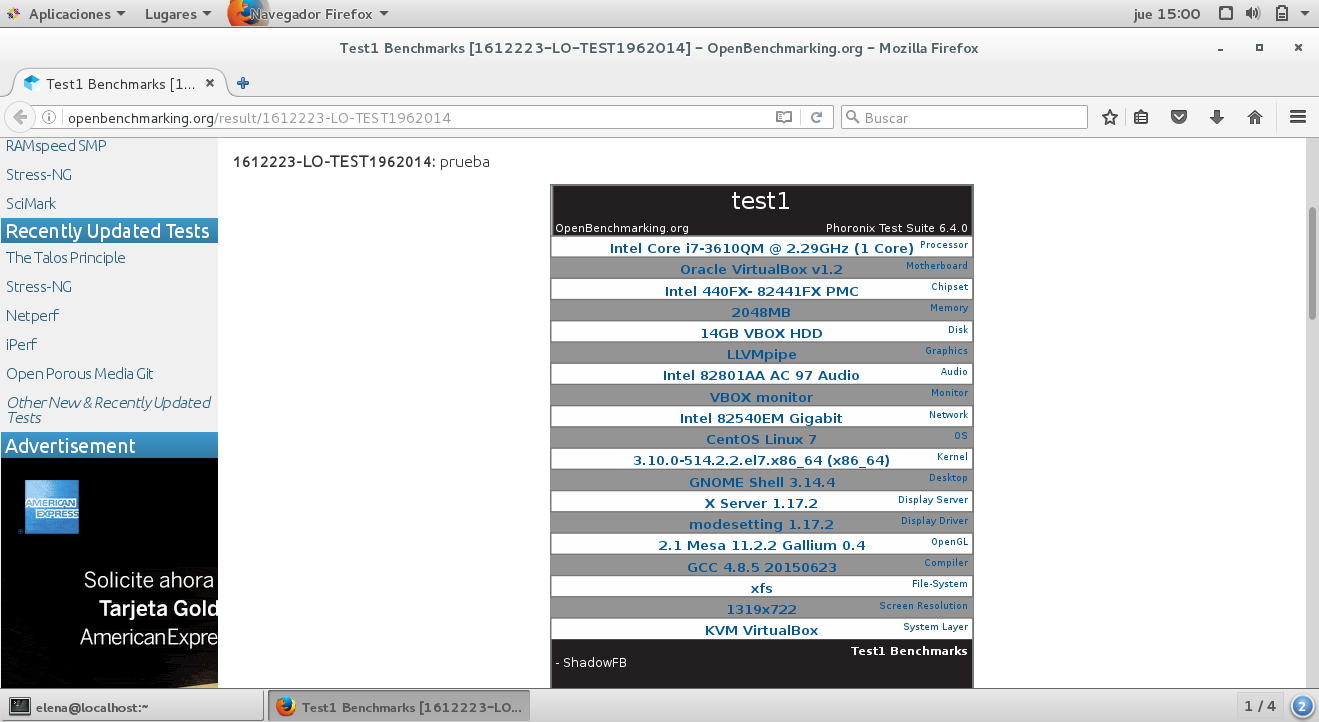
\includegraphics[width=14.7cm]{./img/ejercicio1_14.png} 	
	\caption{CentOS, Phoronix Suite, resultado de benchmark GLmark2.} \label{fig:ejercicio1_14}
\end{figure}

\begin{figure}[H] 
	\centering
	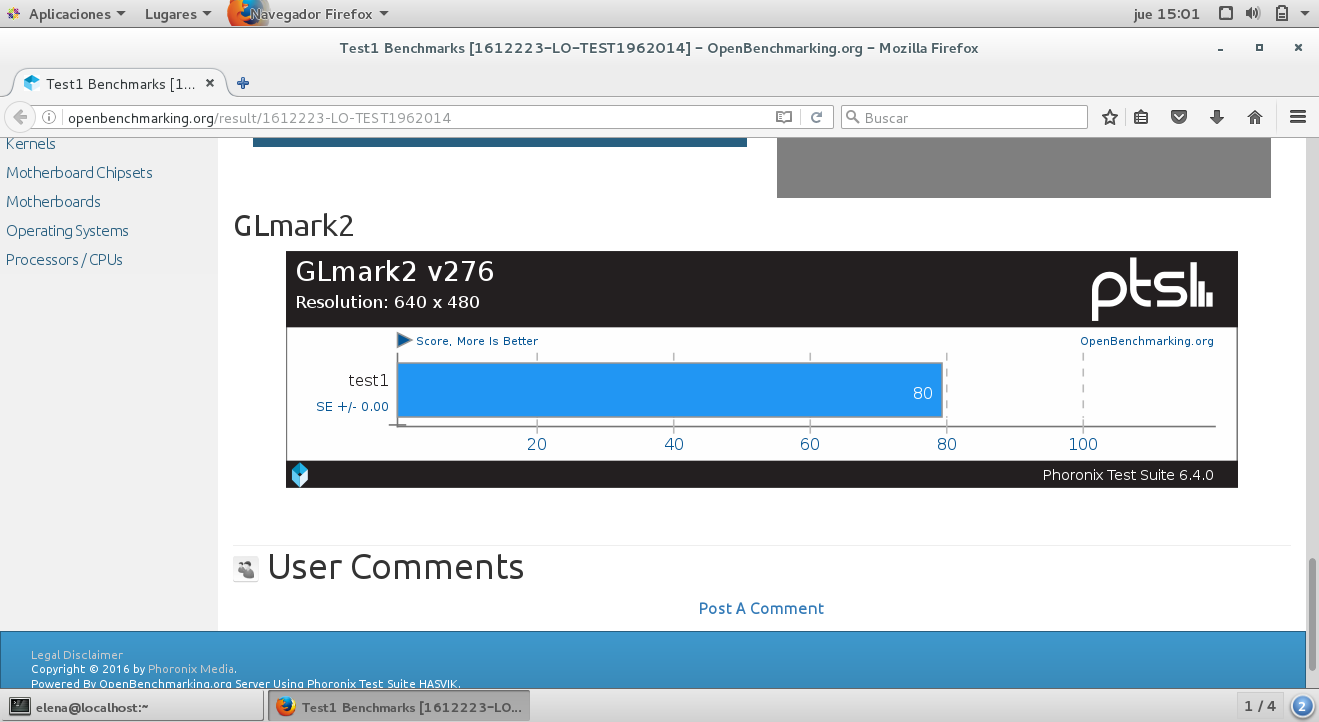
\includegraphics[width=14.7cm]{./img/ejercicio1_15.png} 	
	\caption{CentOS, Phoronix Suite, resultado de benchmark GLmark2.} \label{fig:ejercicio1_15}
\end{figure}

%----------------------------------------------------------------------------------------
%	Cuestión 2
%----------------------------------------------------------------------------------------

\section{Cuestión 2:}

\subsection{De los parámetros que le podemos pasar al comando ¿Qué significa -c 5? ¿y -n 100? Monitorice la ejecución de ab contra alguna máquina (cualquiera) ¿cuántas ``tareas'' crea ab en el cliente?}

Tal y como se indica en el \texttt{man} de \texttt{ab} la opción \texttt{-c 5} indica que se podrán ejecutar concurrentemente 5 solicitudes y la opción \texttt{-n 100} significa que se harán 100 peticiones en el benchmarking actual. \\

He monitorizado la ejecución de \texttt{ab} desde una máquina virtual con CentOS hacia otra con Windows Server, el resultado de la ejecución se muestra en las figuras \ref{fig:ejercicio2_1} y \ref{fig:ejercicio2_2}. El comando \texttt{ab} crea 1 tarea en el cliente como se muestra en la figura \ref{fig:ejercicio2_3}. En el servidor se puede ver un claro aumento del uso de la CPU durante la ejecución de \texttt{ab} (figura \ref{fig:ejercicio2_4}).

\begin{figure}[H] 
	\centering
	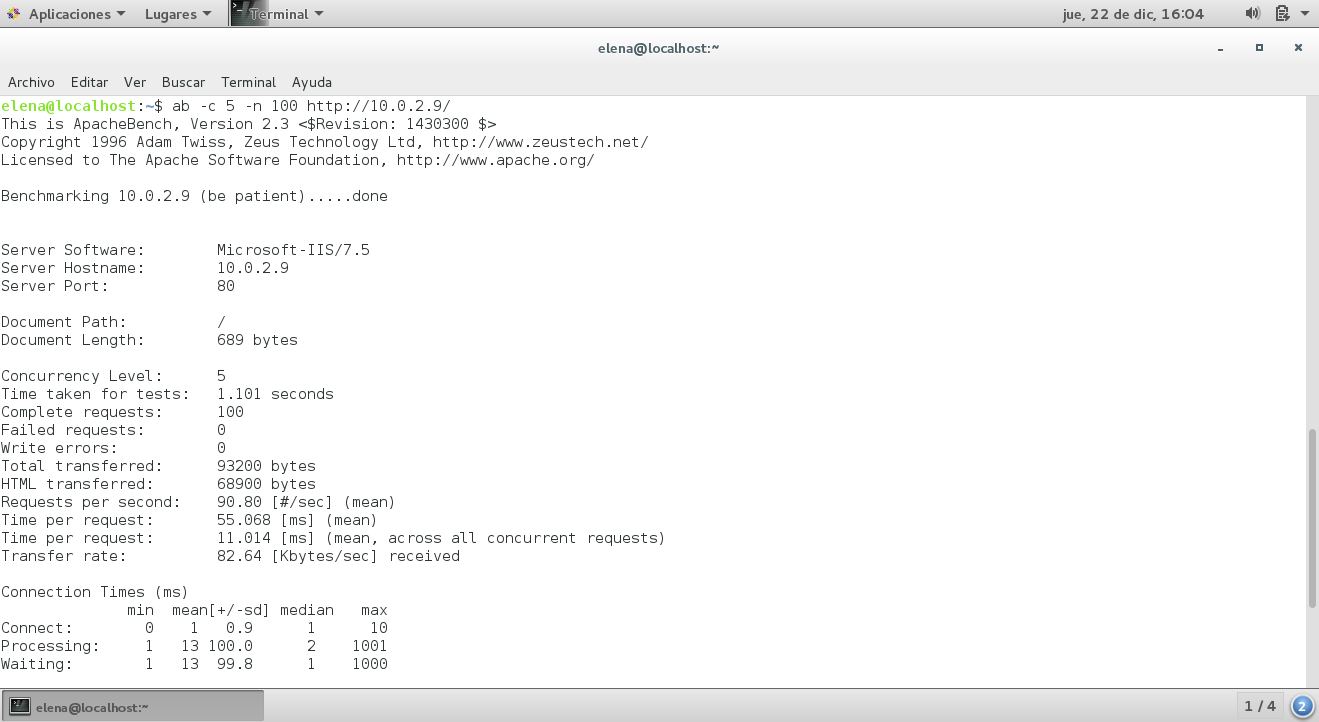
\includegraphics[width=14.7cm]{./img/ejercicio2_1.png} 	
	\caption{CentOS, ab contra Windows Server.} \label{fig:ejercicio2_1}
\end{figure}

\begin{figure}[H] 
	\centering
	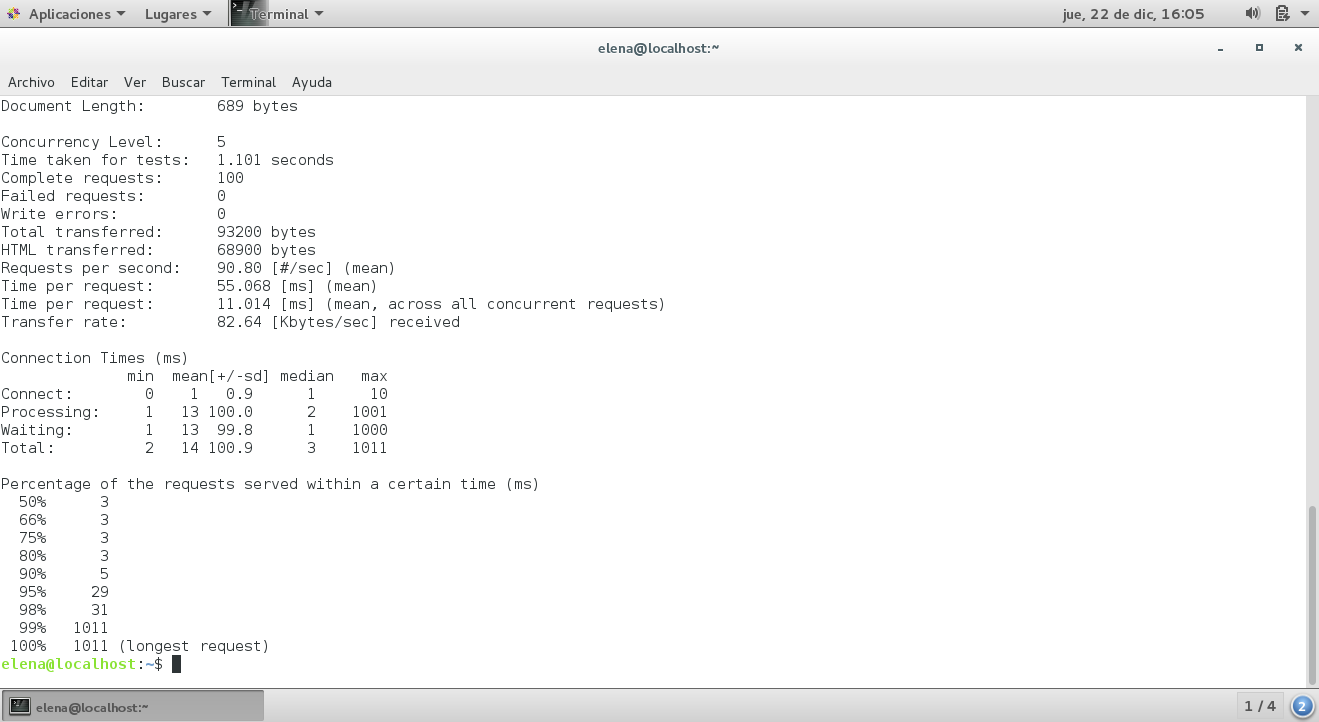
\includegraphics[width=14.7cm]{./img/ejercicio2_2.png} 	
	\caption{CentOS, ab contra Windows Server.} \label{fig:ejercicio2_2}
\end{figure}

\begin{figure}[H] 
	\centering
	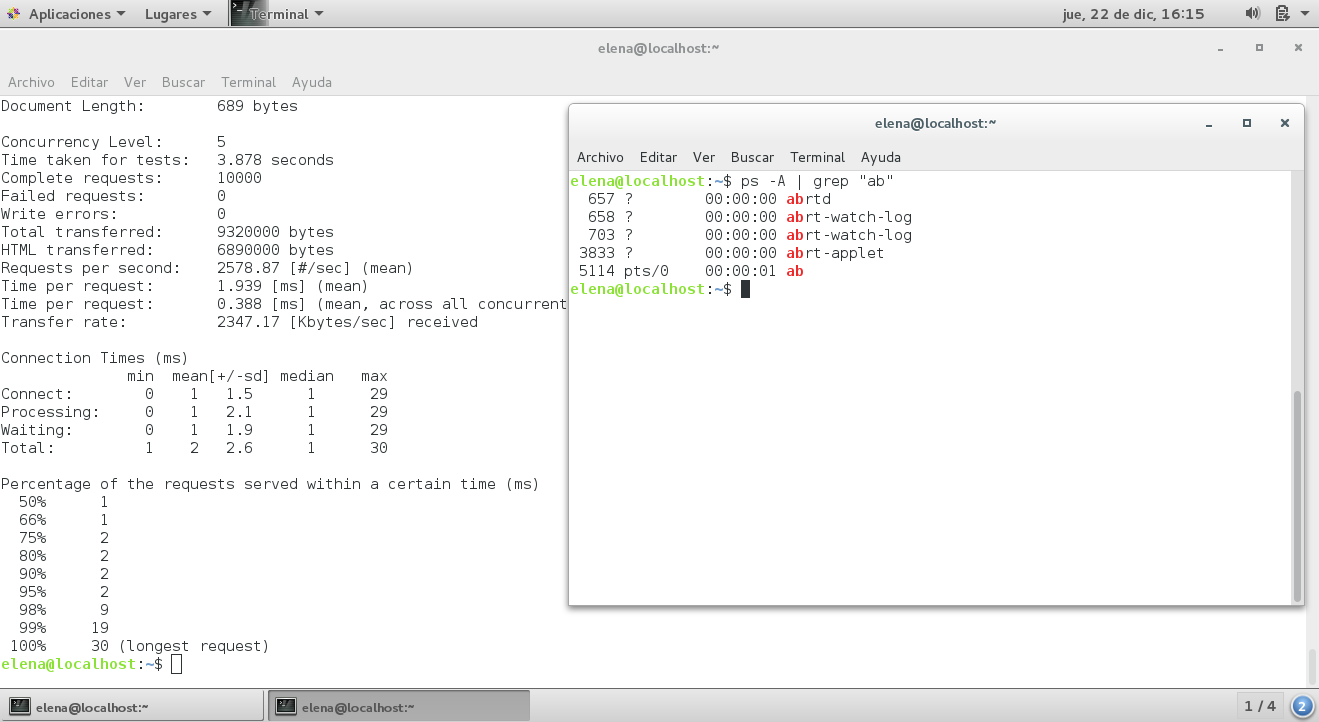
\includegraphics[width=14.7cm]{./img/ejercicio2_3.png} 	
	\caption{CentOS, número de tareas de ab.} \label{fig:ejercicio2_3}
\end{figure}

\begin{figure}[H] 
	\centering
	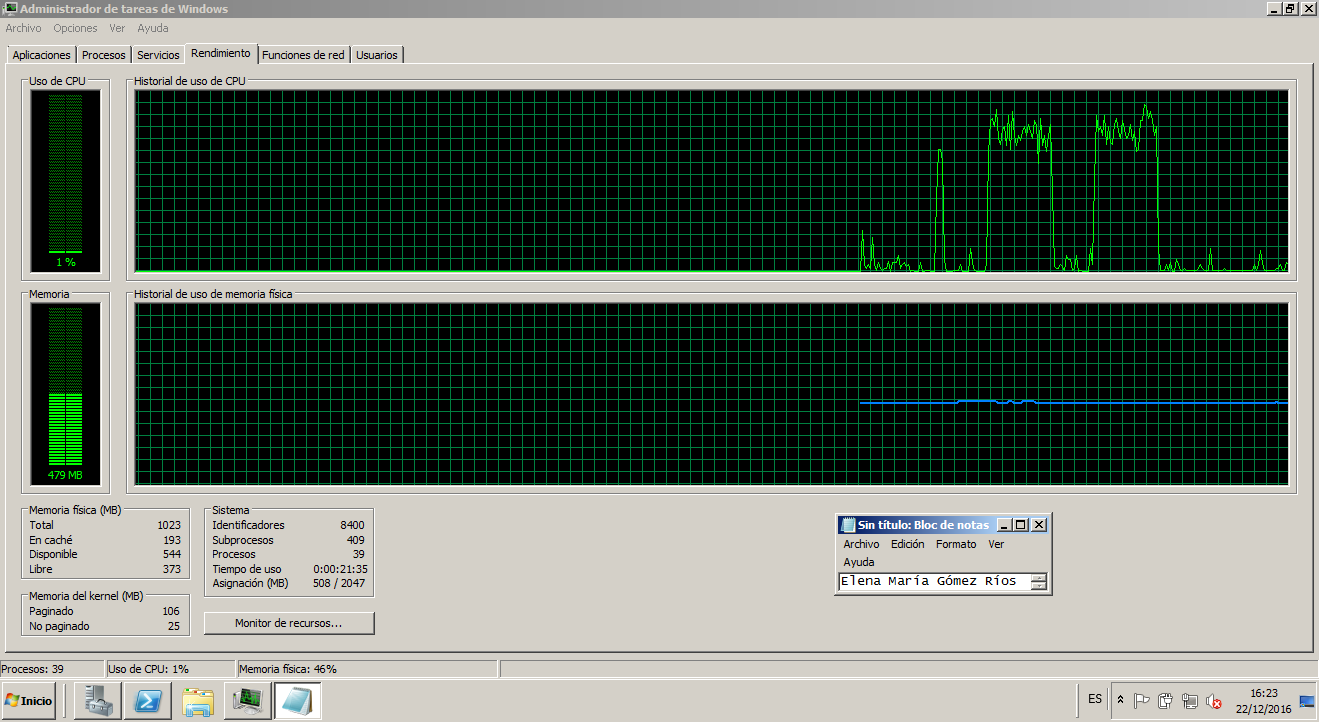
\includegraphics[width=14.7cm]{./img/ejercicio2_4.png} 	
	\caption{Windows, Adminitrador de tareas durante ejecución ab desde CentOS.} \label{fig:ejercicio2_4}
\end{figure}


%----------------------------------------------------------------------------------------
%	Cuestión 3
%----------------------------------------------------------------------------------------

\section{Cuestión 3:}

\subsection{Ejecute ab contra a las tres máquinas virtuales (desde el SO anfitrión a las máquina virtuales de la red local) una a una (arrancadas por separado).¿Cuál es la que proporciona mejores resultados? Muestre y coméntelos. (Use como máquina de referencia Ubuntu Server para la comparativa).}

En primer lugar comentar que este ejercicio lo voy a realizar desde una máquina virtual CentOS en vez de utilizar el SO anfitrión ya que tengo un problema con los puertos, como ya dije en prácticas anteriores, y me es imposible realizar la redirección de puertos de VirtualBox.\\

En primer lugar voy a ejecutar \texttt{ab} contra Windows, los resultados se muestran en las figuras \ref{fig:ejercicio3_1} y \ref{fig:ejercicio3_2}. Para hacerlo contra CentOS he tenido que desactivar el firewall como se muestra en la figura \ref{fig:ejercicio3_3} ya que por defecto el firewall bloquea todo el tráfico impidiendo ejecutar \texttt{ab}. Los resultados de \texttt{ab} contra CentOS se muestran en las figuras \ref{fig:ejercicio3_4} y \ref{fig:ejercicio3_5}. Por último he realizado el test \texttt{ab} contra Ubuntu Server como se muestra en las figuras \ref{fig:ejercicio3_6} y \ref{fig:ejercicio3_7}. Igualmente en Ubuntu he tenido que deshabilitar el firewall con el comando \texttt{sudo ufw disable}.\\

Para una fácil comparación entre los resultados de \texttt{ab} contra las diferentes máquinas virtuales voy a mostrar los resultados en la tabla \ref{comparativa_ab}.

\begin{table}[H]
\centering
\small
\setlength\tabcolsep{2pt}
\caption{Resultados de ab.}
\label{comparativa_ab}
\begin{tabular}{|c|c|c|c|c|c|}
\hline
\textbf{SO}      & \textbf{Tamaño web} & \textbf{Tiempo (s)} & \textbf{Datos Transferidos} & \textbf{Respuestas/s} & \textbf{Ratio Transferencia} \\ \hline
\textbf{CentOS}  & 4897 bytes          & 64.347              & 493.90 MB                   & 1554.08               & 7859.94 KB/s                      \\ \hline
\textbf{Ubuntu}  & 11510 bytes         & 54.763              & 1123.71 MB                  & 1826.06               & 21012.13 KB/s                     \\ \hline
\textbf{Windows} & 689 bytes           & 31.895              & 88.882 MB                   & 3135.33               & 2853.64 KB/s                    \\ \hline
\end{tabular}
\end{table}


Como se puede observar mirando la columna correspondiente al ratio de transferencia, la máquina virtual que proporciona mejores resultados es Ubuntu, seguida de CentOS y por último Windows. Ubuntu tiene un ratio de transferencia 7.3632 veces mejor que Windows, y 2.67 veces mejor que CentOS.


\begin{figure}[H] 
	\centering
	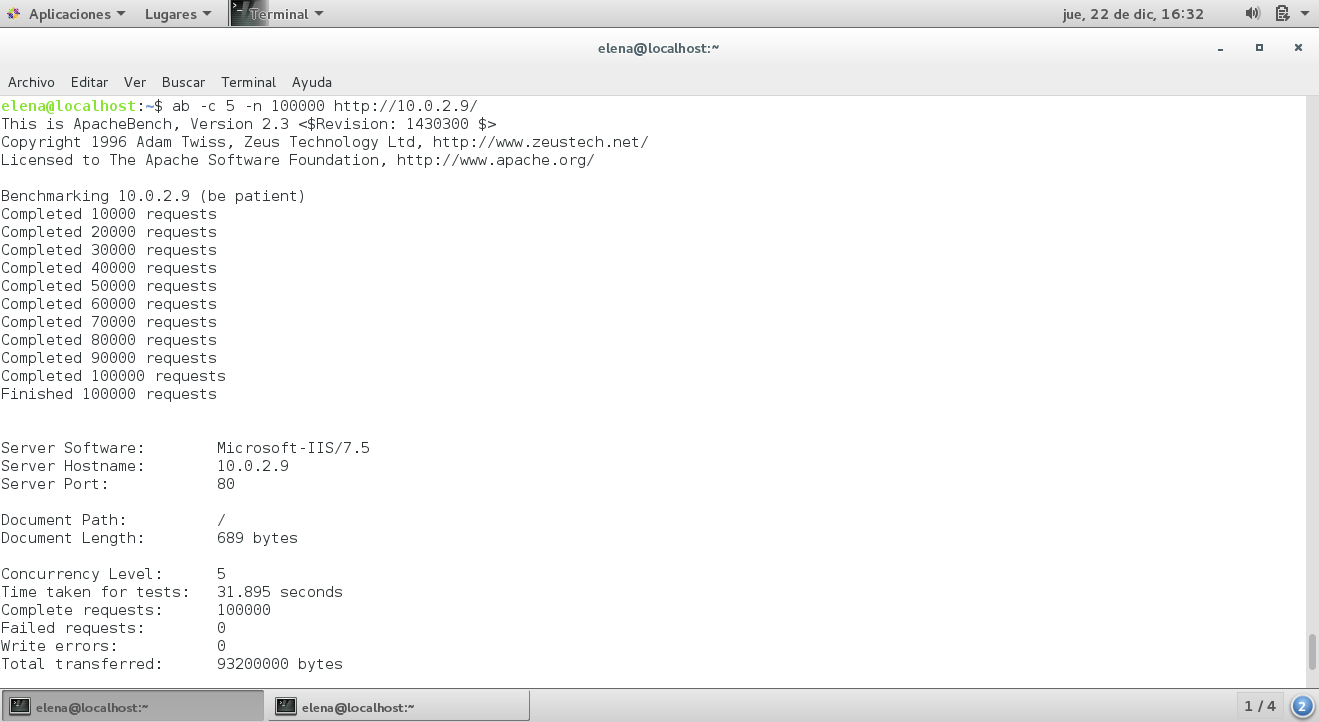
\includegraphics[width=14.7cm]{./img/ejercicio3_1.png} 	
	\caption{CentOS, resultado ab contra Windows.} \label{fig:ejercicio3_1}
\end{figure}

\begin{figure}[H] 
	\centering
	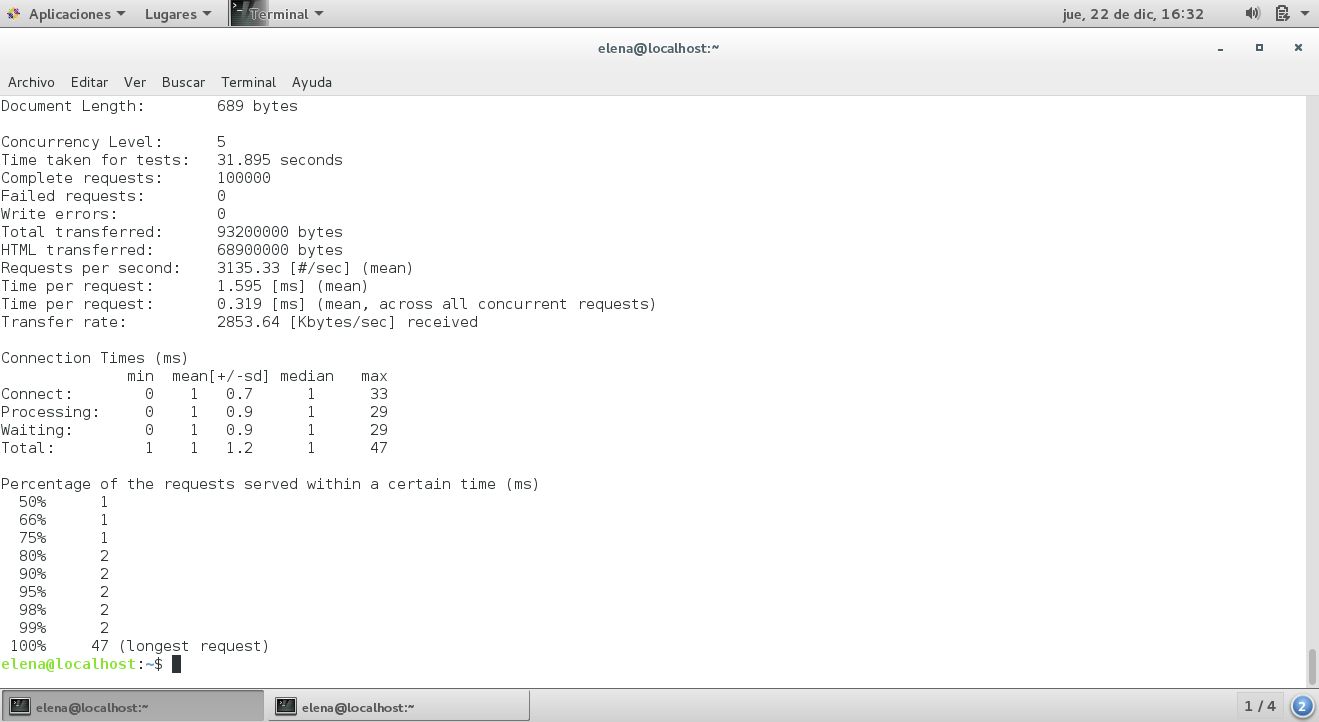
\includegraphics[width=14.7cm]{./img/ejercicio3_2.png} 	
	\caption{CentOS, resultado ab contra Windows.} \label{fig:ejercicio3_2}
\end{figure}

\begin{figure}[H] 
	\centering
	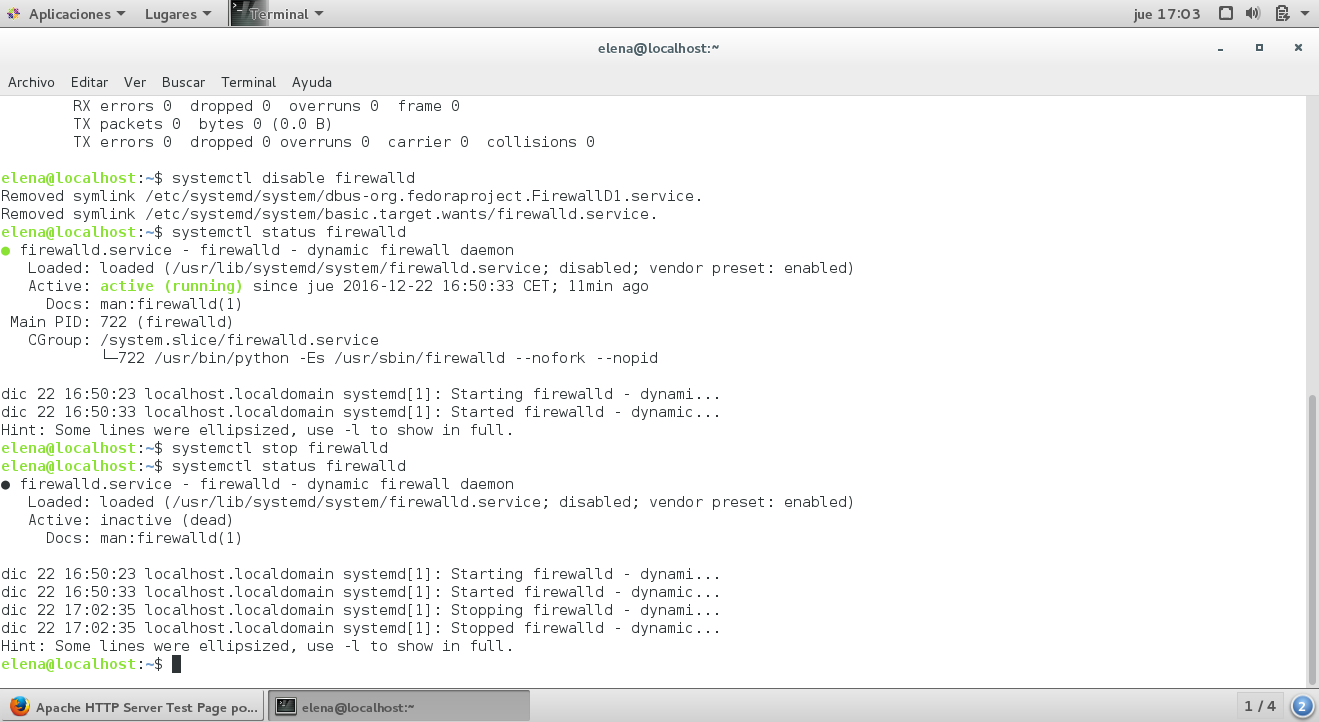
\includegraphics[width=14.7cm]{./img/ejercicio3_3.png} 	
	\caption{CentOS, desactivación del firewall.} \label{fig:ejercicio3_3}
\end{figure}

\begin{figure}[H] 
	\centering
	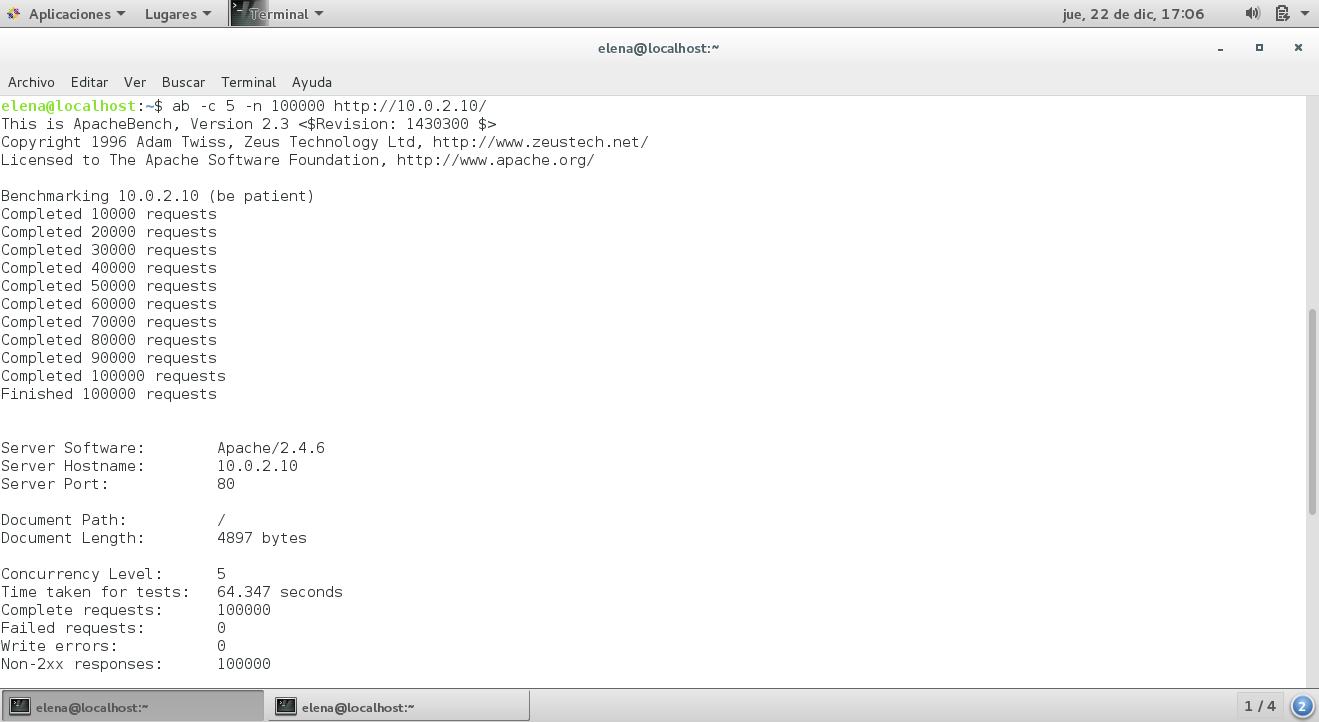
\includegraphics[width=14.7cm]{./img/ejercicio3_4.png} 	
	\caption{CentOS, resultado ab contra CentOS.} \label{fig:ejercicio3_4}
\end{figure}

\begin{figure}[H] 
	\centering
	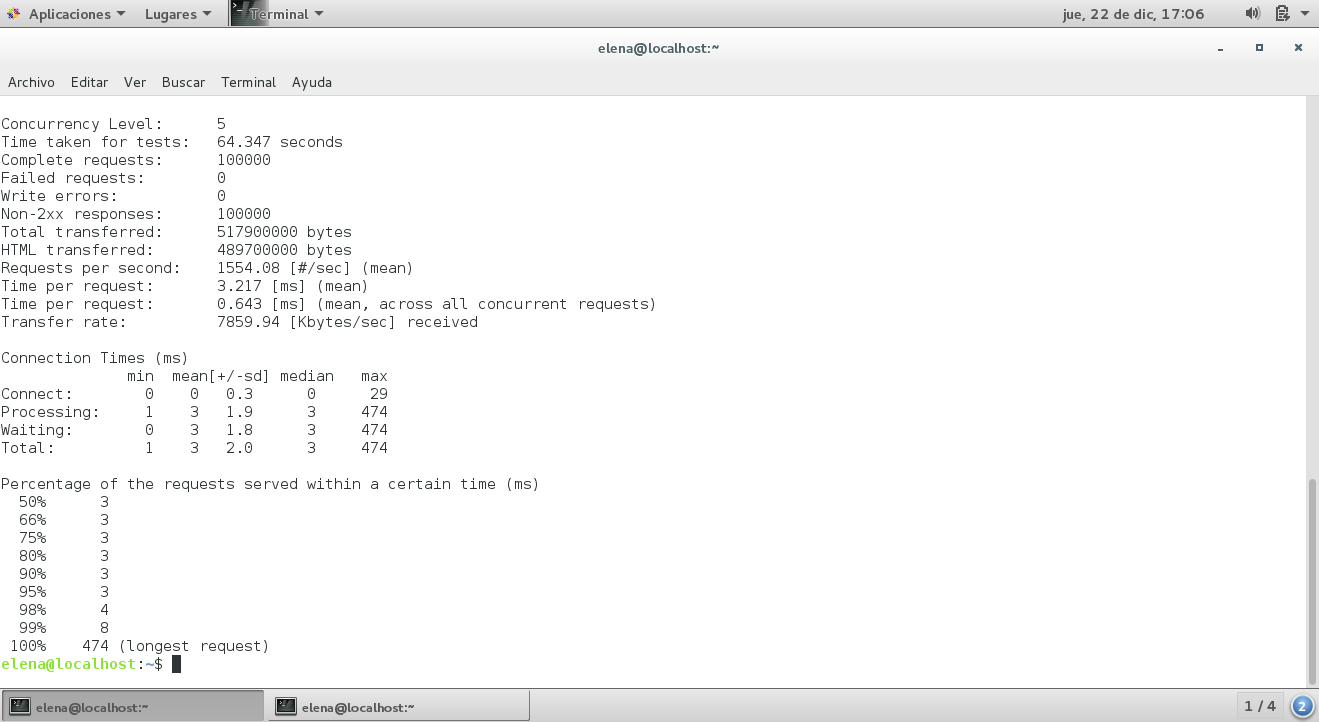
\includegraphics[width=14.7cm]{./img/ejercicio3_5.png} 	
	\caption{CentOS, resultado ab contra CentOS.} \label{fig:ejercicio3_5}
\end{figure}

\begin{figure}[H] 
	\centering
	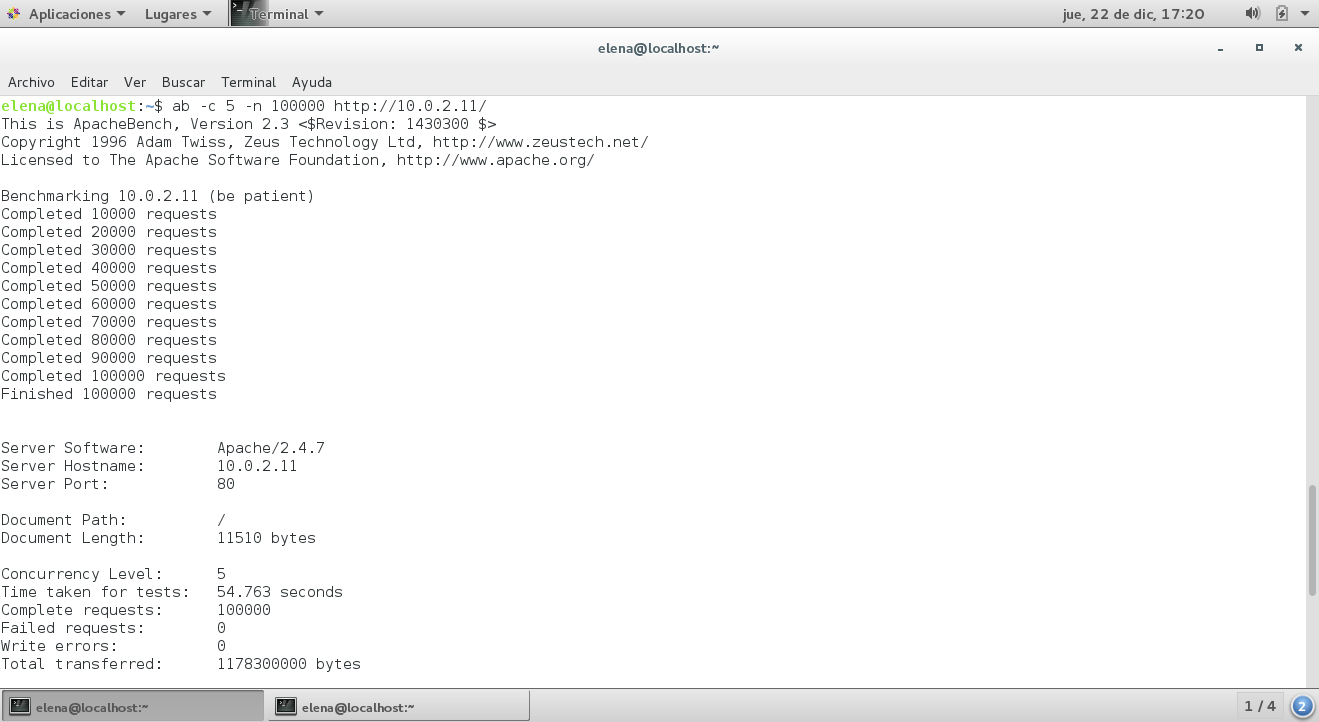
\includegraphics[width=14.7cm]{./img/ejercicio3_6.png} 	
	\caption{CentOS, resultado ab contra Ubuntu Server.} \label{fig:ejercicio3_6}
\end{figure}

\begin{figure}[H] 
	\centering
	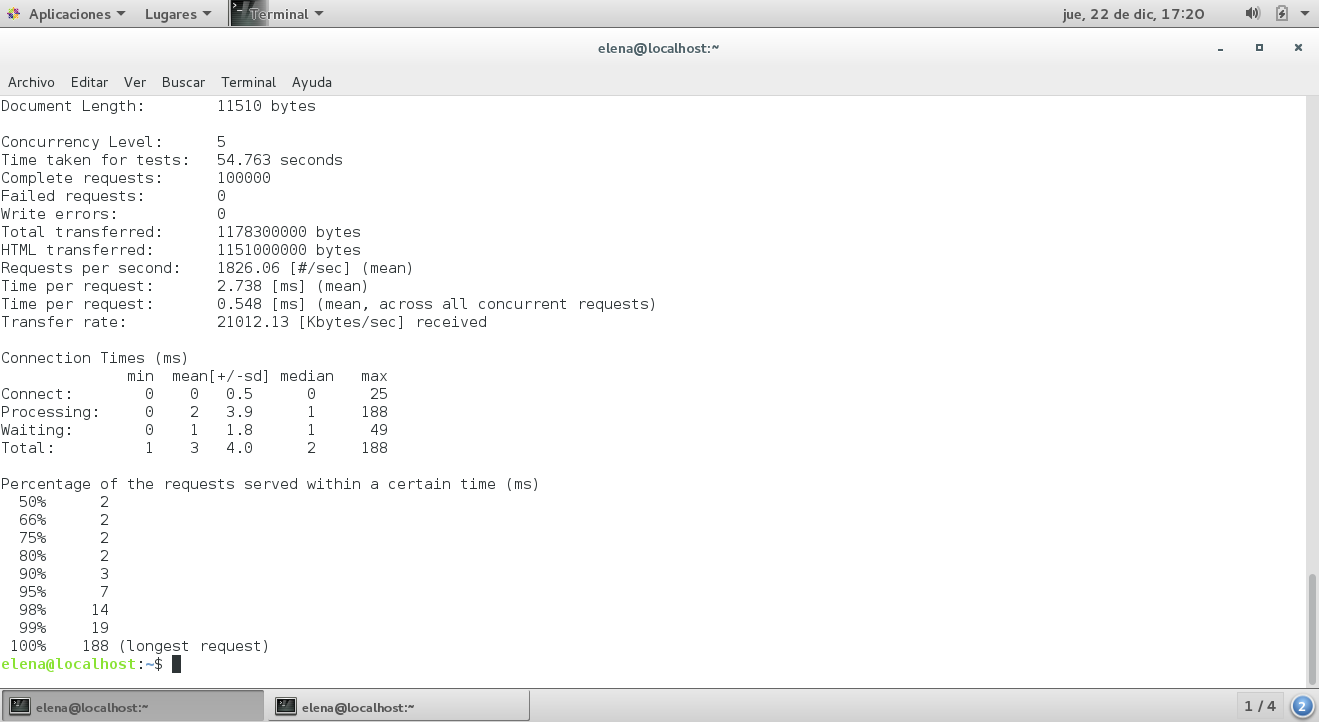
\includegraphics[width=14.7cm]{./img/ejercicio3_7.png} 	
	\caption{CentOS, resultado ab contra Ubuntu Server.} \label{fig:ejercicio3_7}
\end{figure}



%----------------------------------------------------------------------------------------
%  Cuestión opcional 1:
%----------------------------------------------------------------------------------------

\section{Cuestión opcional 1:}

\subsection{¿Qué es Scala? Instale Gatling y pruebe los escenarios por defecto.}

Tal y como se dice en la página oficial de Scala \cite{Scala}, Scala (``Scalable Language'') es un lenguaje de programación orientado a objetos y cuenta con todas sus características principales. Utiliza una sintaxis concisa, elegante e incluso permite agregar nuevas operaciones a las clases existentes, no importa si vienen de Scala o Java.\\

Para instalar Gatling he seguido el tutorial de su página oficial \cite{Gatling}. Primero debemos descargarnos el paquete de Gatling que proporciona la página web y lo descomprimimos (figura \ref{fig:opcional1_1}). Para ejecutar Gatling debemos ejecutar el archivo, \texttt{gatling.sh}, que se encuentra en la carpeta \texttt{/bin} de este paquete (figura \ref{fig:opcional1_2}). \\

Nos da la opción de elegir entre 6 simulaciones, por ejemplo seleccionamos la opción 0 ``computerdatabase.BasicSimulation'', la cual nos muestra la información que aparece en la figura \ref{fig:opcional1_3}, y podemos verlos más cómodamente en la web de resultados que crea Gatling, como se muestra en la figura \ref{fig:opcional1_4}.\\

También podemos seleccionar alguno de los otros escenarios por defecto como ``computerdatabase.advanced.AdvancedSimulationStep01'', el cual nos devuelve los datos de las figuras \ref{fig:opcional1_5} y \ref{fig:opcional1_6}. O el escenario ``computerdatabase.advanced.AdvancedSimulationStep05'', el cual nos devuelve los datos de las figuras \ref{fig:opcional1_7} y \ref{fig:opcional1_8}.



\begin{figure}[H] 
	\centering
	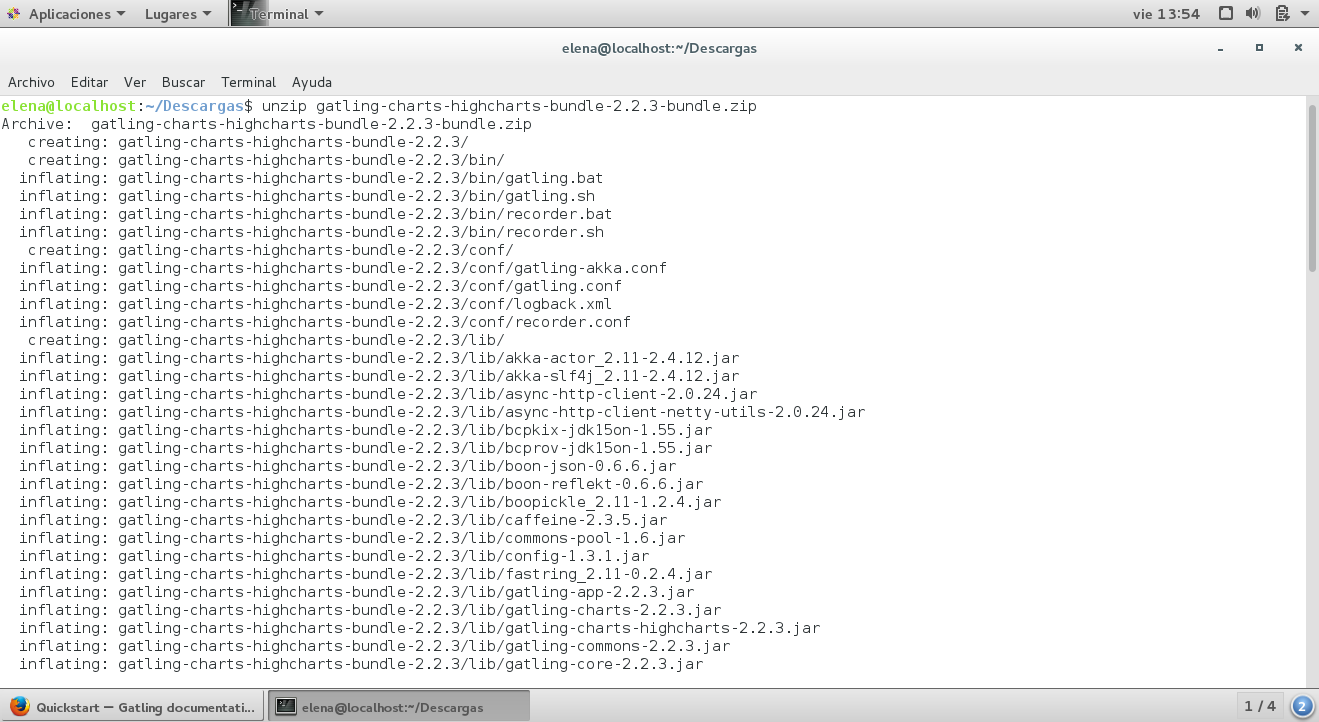
\includegraphics[width=14.7cm]{./img/opcional1_1.png} 	
	\caption{CentOS, instalación de Gatling.} \label{fig:opcional1_1}
\end{figure}

\begin{figure}[H] 
	\centering
	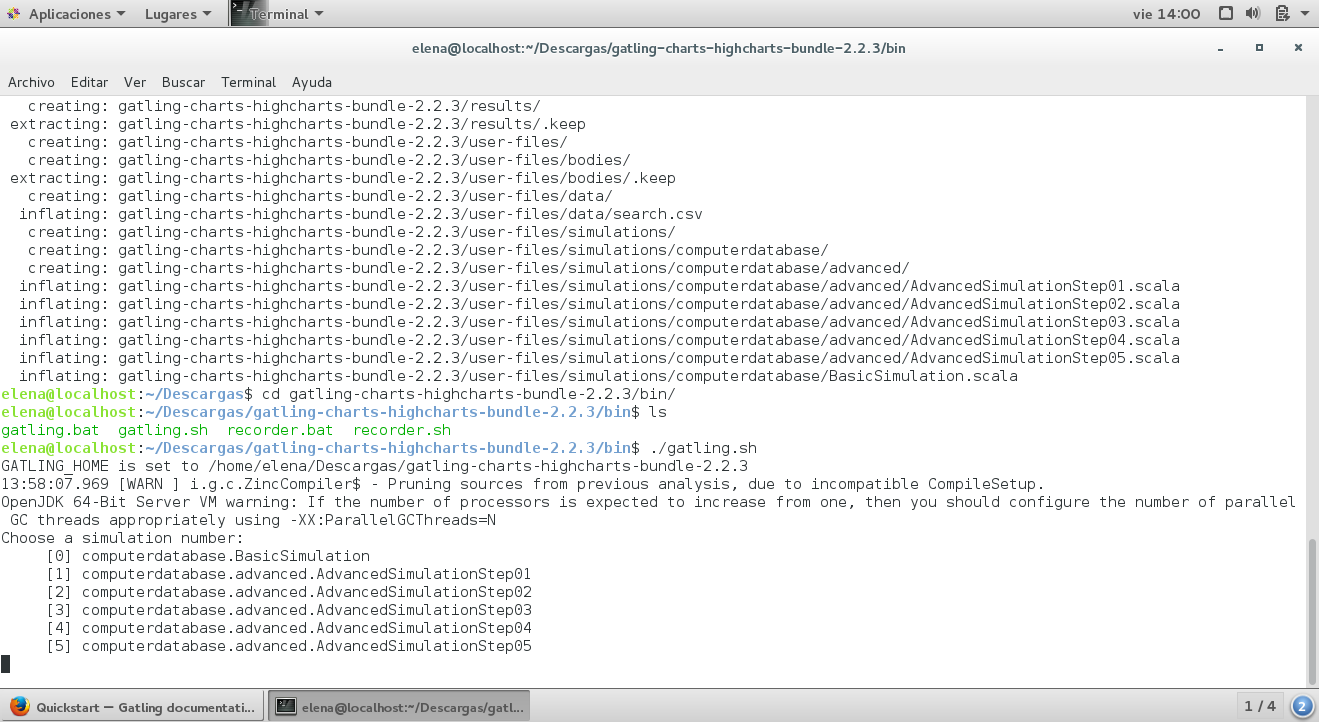
\includegraphics[width=14.7cm]{./img/opcional1_2.png} 	
	\caption{CentOS, ejecución de Gatling.} \label{fig:opcional1_2}
\end{figure}

\begin{figure}[H] 
	\centering
	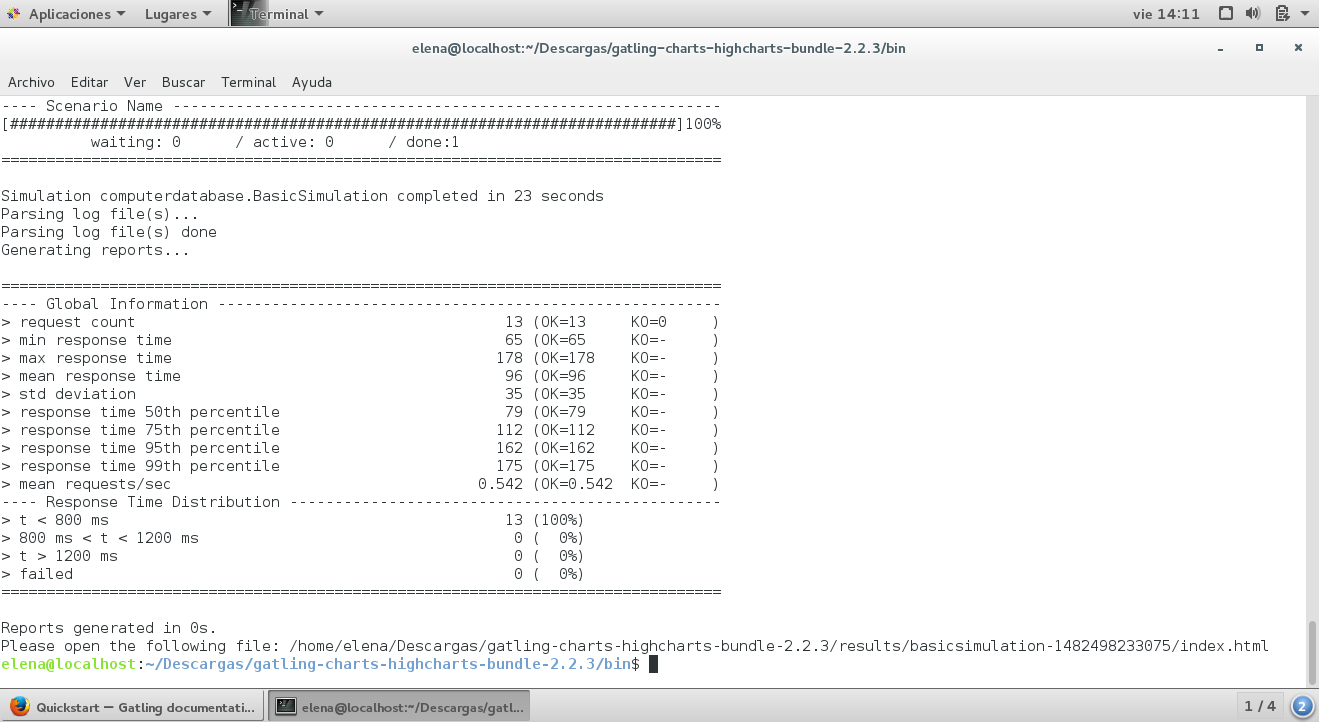
\includegraphics[width=14.7cm]{./img/opcional1_3.png} 	
	\caption{CentOS, resultados de Gatling, escenario 0.} \label{fig:opcional1_3}
\end{figure}

\begin{figure}[H] 
	\centering
	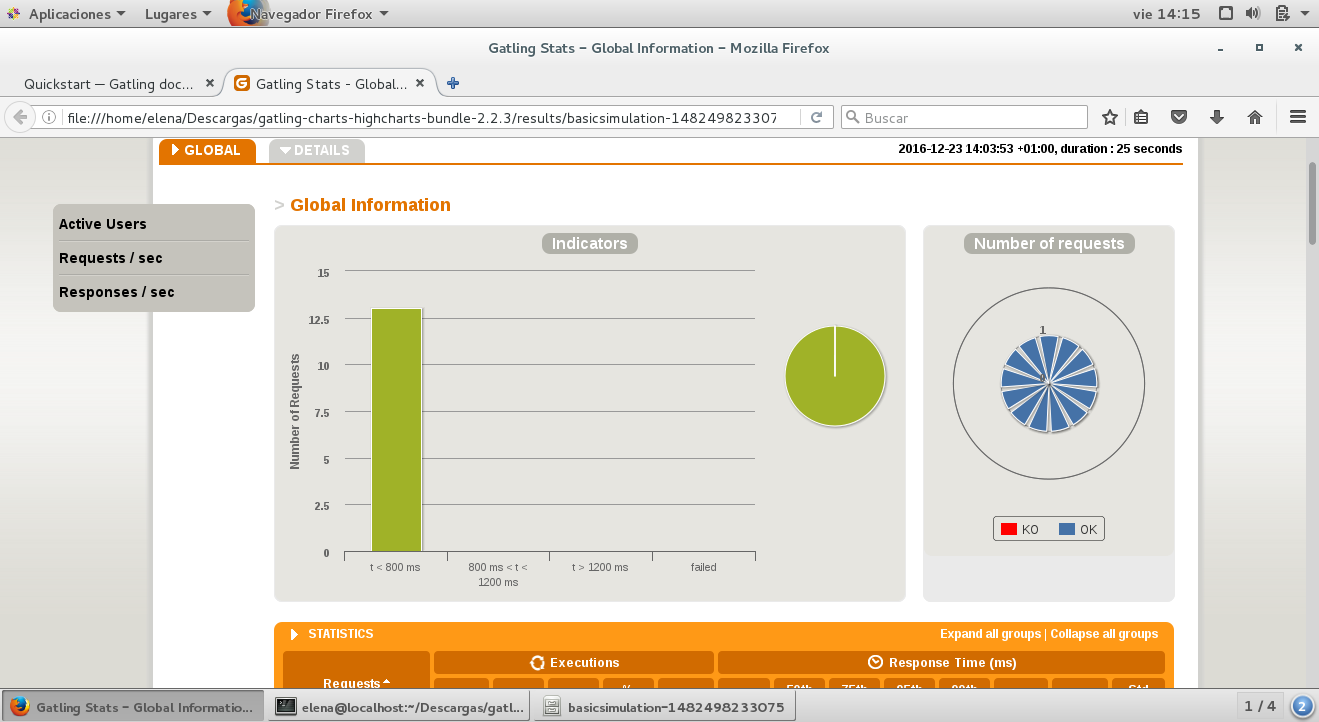
\includegraphics[width=14.7cm]{./img/opcional1_4.png} 	
	\caption{CentOS, resultados de Gatling, escenario 0.} \label{fig:opcional1_4}
\end{figure}

\begin{figure}[H] 
	\centering
	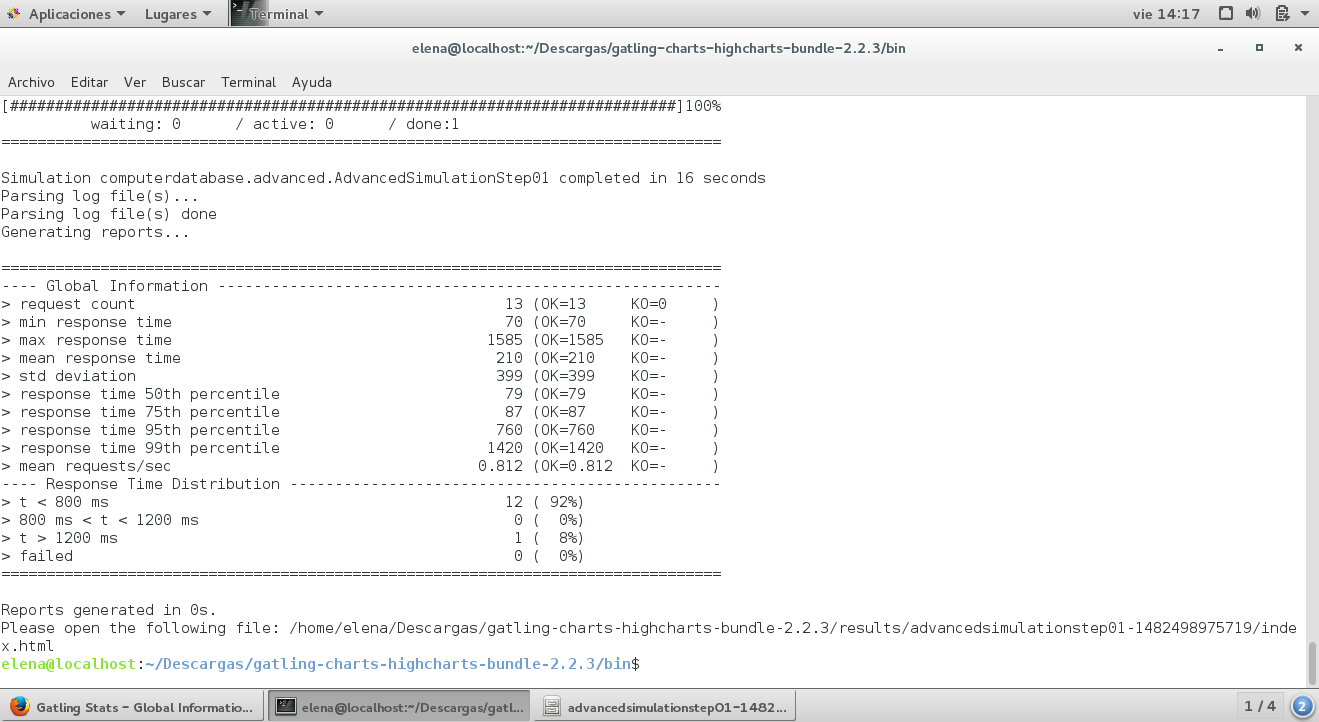
\includegraphics[width=14.7cm]{./img/opcional1_5.png} 	
	\caption{CentOS, resultados de Gatling, escenario 1.} \label{fig:opcional1_5}
\end{figure}

\begin{figure}[H] 
	\centering
	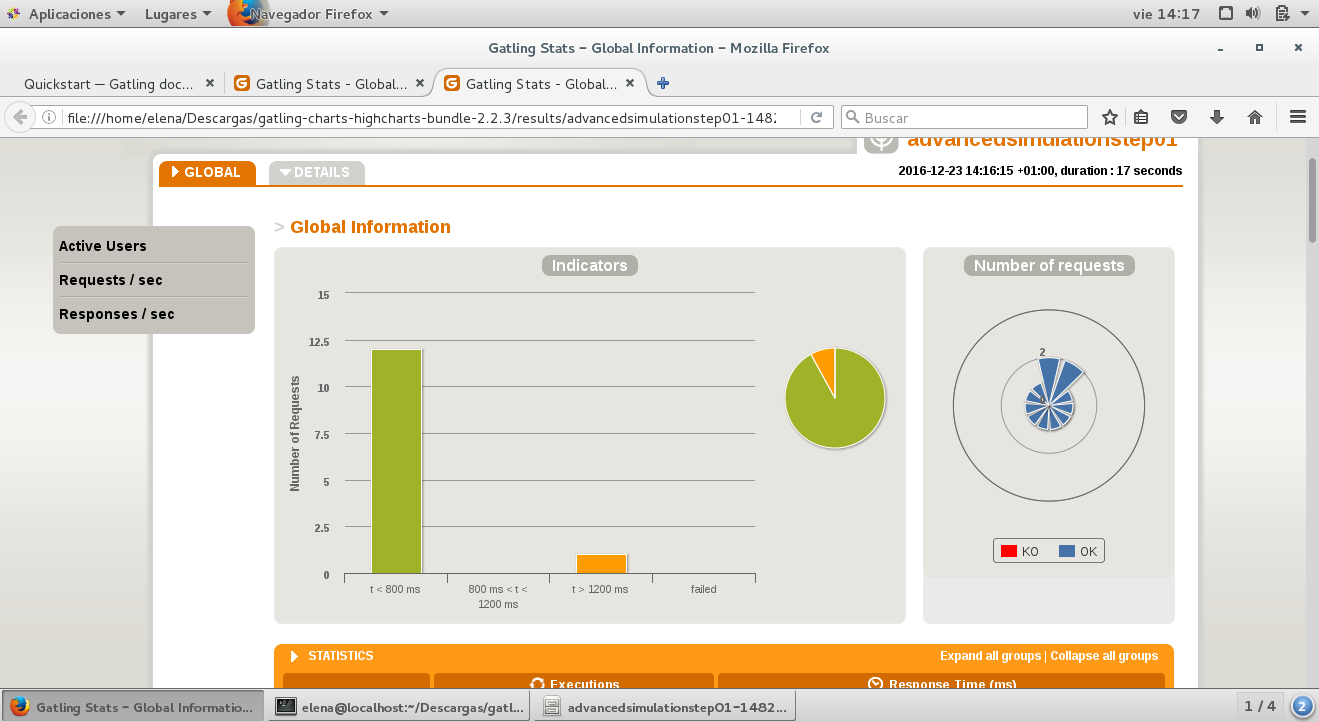
\includegraphics[width=14.7cm]{./img/opcional1_6.png} 	
	\caption{CentOS, resultados de Gatling, escenario 1} \label{fig:opcional1_6}
\end{figure}

\begin{figure}[H] 
	\centering
	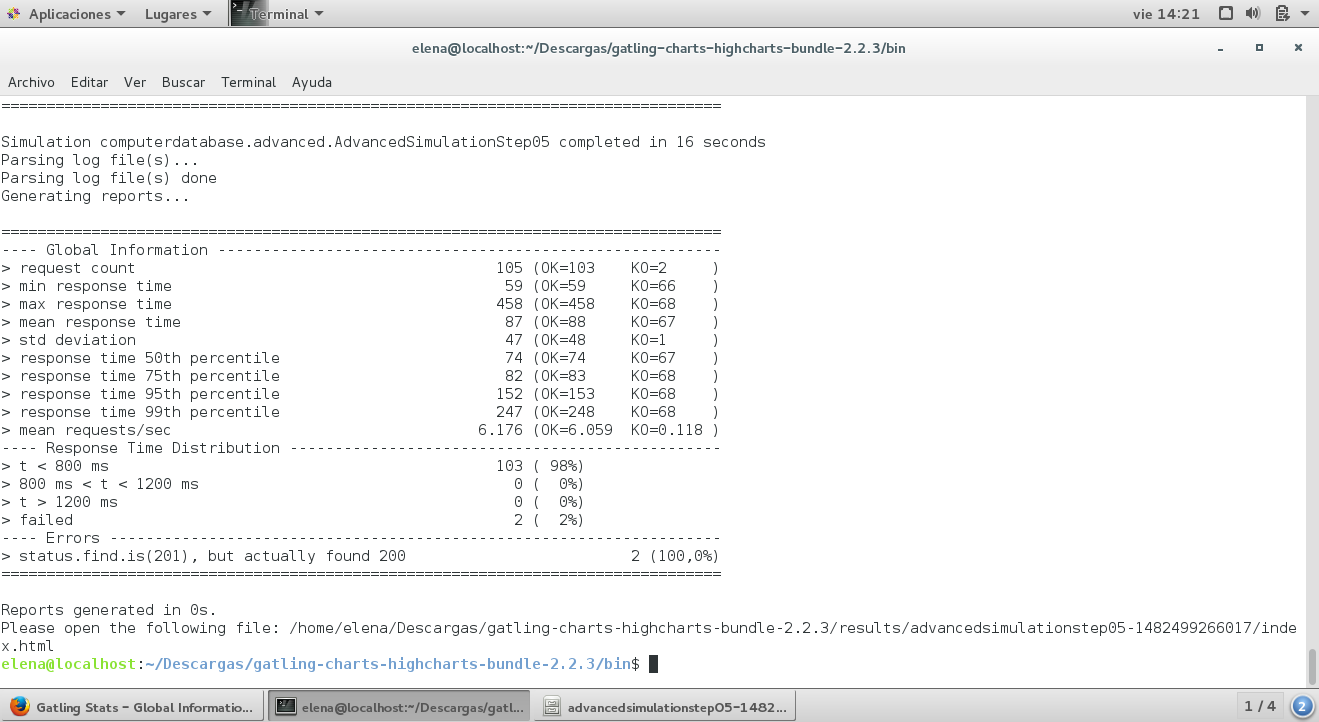
\includegraphics[width=14.7cm]{./img/opcional1_7.png} 	
	\caption{CentOS, resultados de Gatling, escenario 5.} \label{fig:opcional1_7}
\end{figure}

\begin{figure}[H] 
	\centering
	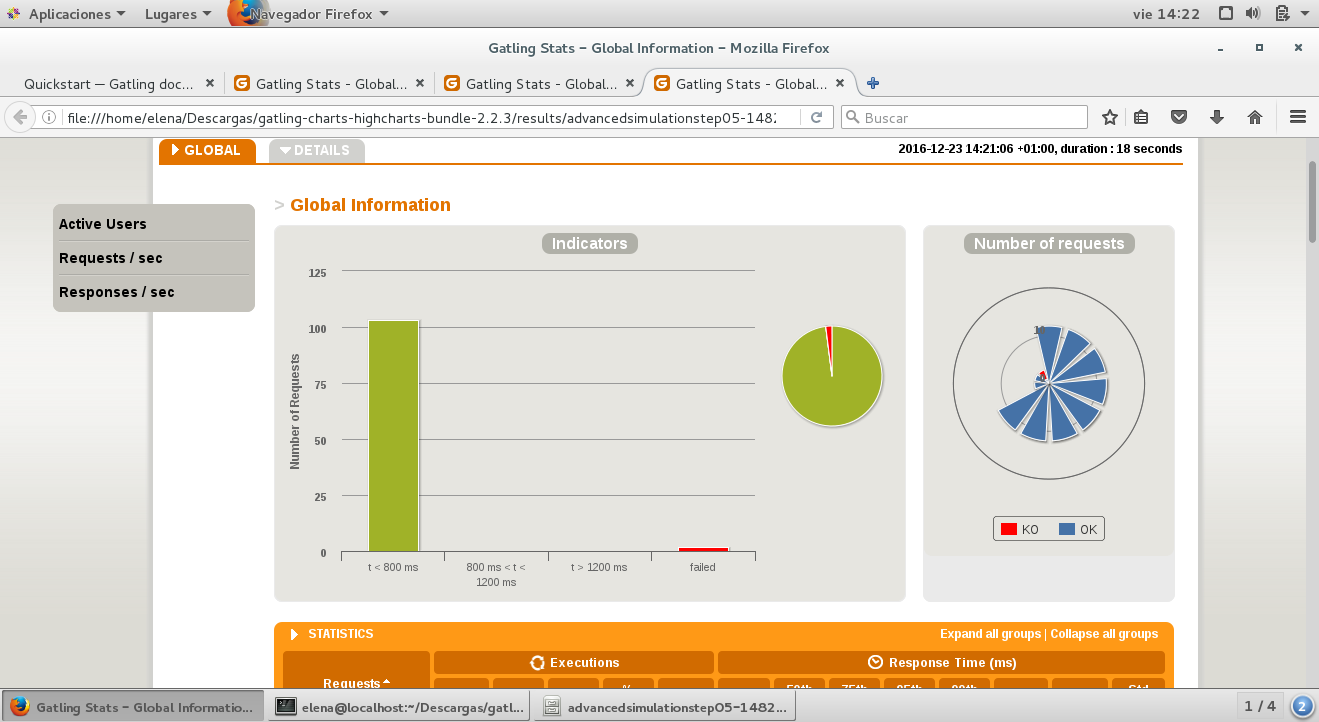
\includegraphics[width=14.7cm]{./img/opcional1_8.png} 	
	\caption{CentOS, resultados de Gatling, escenario 5} \label{fig:opcional1_8}
\end{figure}


%----------------------------------------------------------------------------------------
%	Cuestión 4
%----------------------------------------------------------------------------------------

\section{Cuestión 4:}

\subsection{Instale y siga el tutorial en http://jmeter.apache.org/usermanual/build-web-test-plan.html \cite{ejer4} realizando capturas de pantalla y comentándolas. En vez de usar la web de jmeter, haga el experimento usando sus máquinas virtuales ¿coincide con los resultados de ab?}

Para instalar JMeter nos descargamos el binario .zip de la página oficial, lo descomprimimos y ejecutamos el script \texttt{apache-jmeter-3.1/bin/jmeter}.\\

Lo primero que tenemos que hacer es crear un grupo de hilos, como se muestra en la figura \ref{fig:ejercicio4_1} y nos saldrá algo parecido a la figura \ref{fig:ejercicio4_2} con los valores por defecto. Cambiamos los valores del número de hilos a 5, y contador del bucle a 2, tal y como se muestra en la figura \ref{fig:ejercicio4_3}.\\

Ahora añadimos los valores de las peticiones HTTP por defecto, para ello debemos entrar tal y como se muestra en la figura \ref{fig:ejercicio4_4}, una vez añadidos se mostrará algo similar a la figura \ref{fig:ejercicio4_5} teniendo en cuenta que hemos puesto la ip de nuestra máquina virtual de Ubuntu Server. También podemos añadir un gestor de Cookies de HTTP, como se muestra en la figura \ref{fig:ejercicio4_6}.\\

A continuación añadimos las peticiones HTTP para nuestro test, como se muestra en la figura \ref{fig:ejercicio4_7} con los valores que se muestran en la figura \ref{fig:ejercicio4_8}.\\

Finalmente añadimos una gráfica para ver los resultados de los test creados tal y como se muestra en la figura \ref{fig:ejercicio4_9} y seleccionamos el fichero de salida de JMeter (figura \ref{fig:ejercicio4_10}). Ejecutando el test de JMeter varias veces hacia Ubuntu Server se obtiene la siguiente gráfica (\ref{fig:ejercicio4_11}). Hacemos lo mismo para Windows (figura \ref{fig:ejercicio4_12}) y CentOS (figura \ref{fig:ejercicio4_13}), cambiando la ip en los valores por defecto de las peticiones de HTTP. Para que las gráficas fuesen significativas he cambiado el número de bucles de 2 a 200.\\

Como se puede observar en las gráficas el rendimiento en Ubuntu es 33.5/minuto, en Windows 35,84/minuto y en CentOS 41.039/minuto.


\begin{figure}[H] 
	\centering
	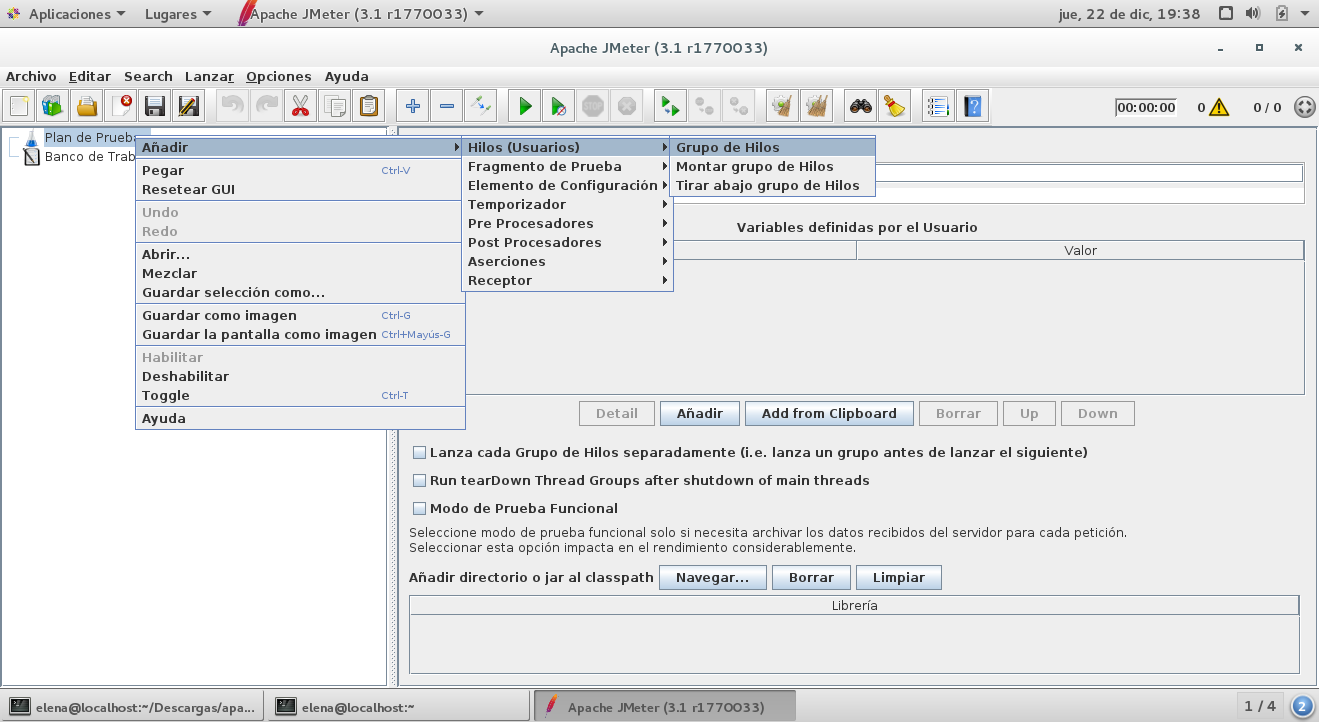
\includegraphics[width=14.7cm]{./img/ejercicio4_1.png} 	
	\caption{CentOS, JMeter - crear grupo de hilos.} \label{fig:ejercicio4_1}
\end{figure}

\begin{figure}[H] 
	\centering
	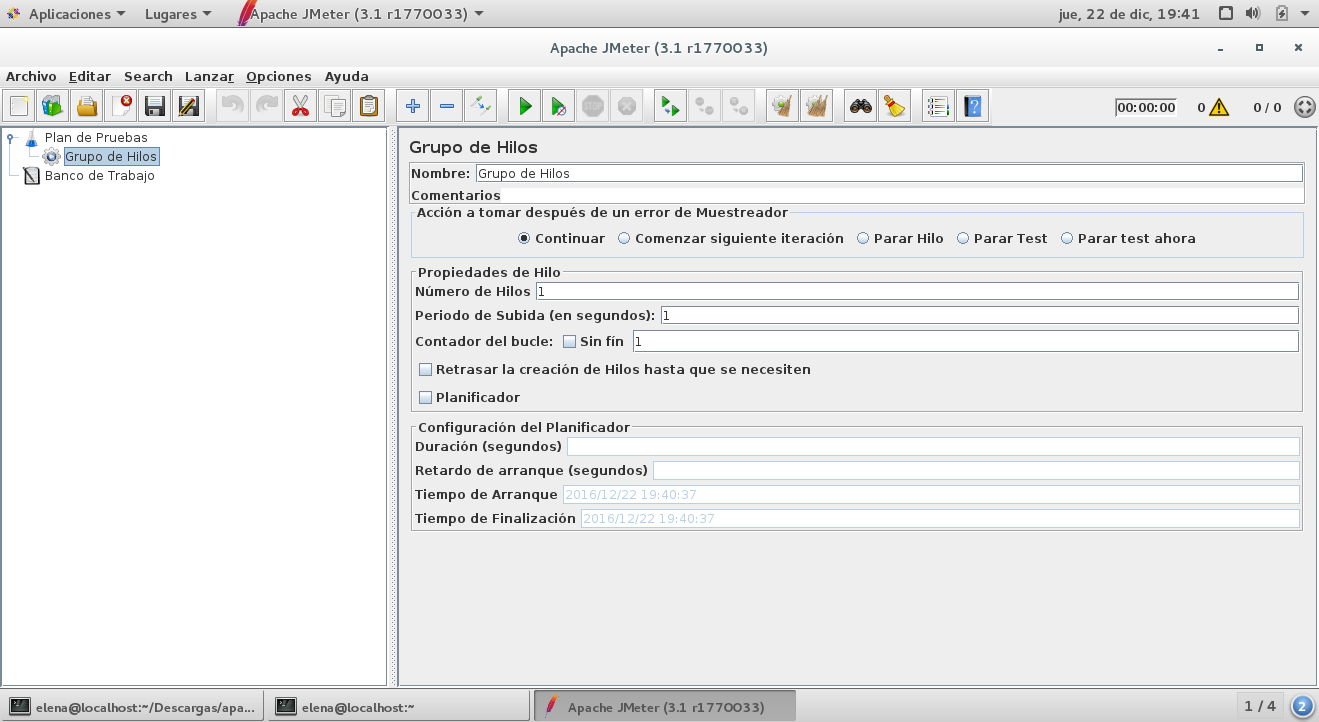
\includegraphics[width=14.7cm]{./img/ejercicio4_2.png} 	
	\caption{CentOS, JMeter - grupo de hilos por defecto.} \label{fig:ejercicio4_2}
\end{figure}

\begin{figure}[H] 
	\centering
	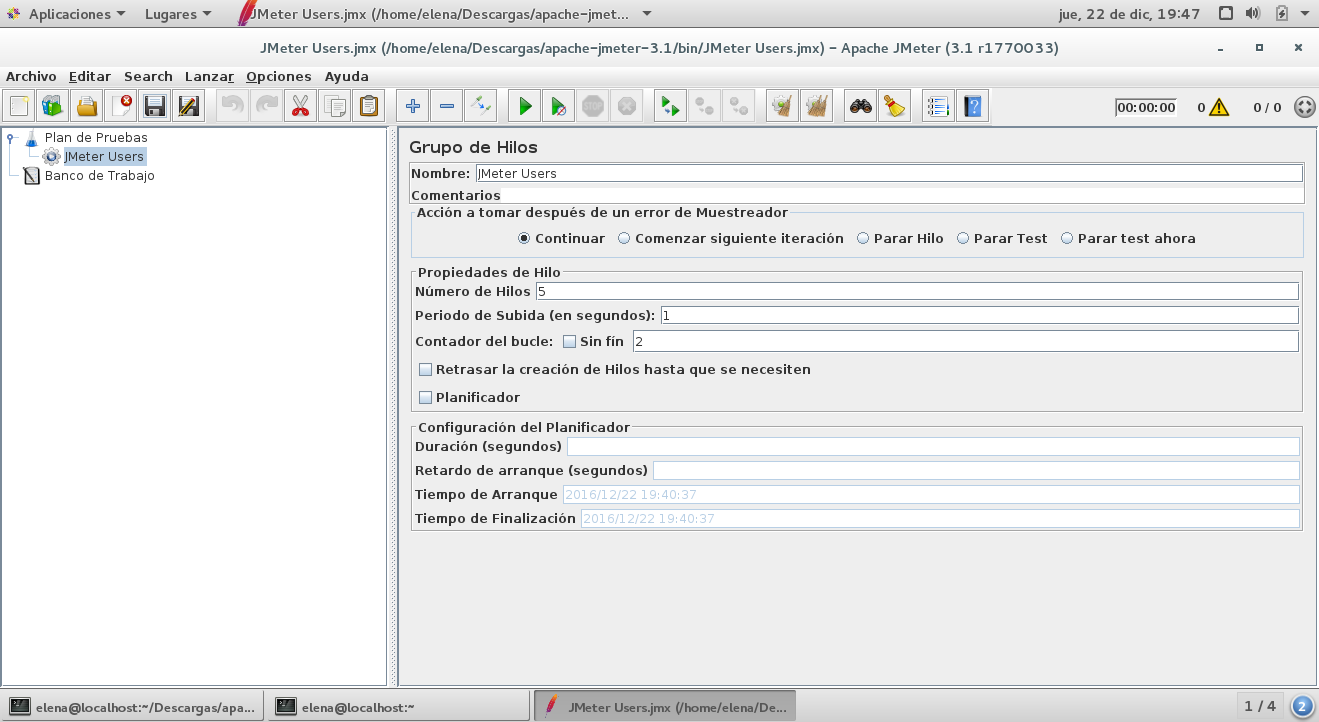
\includegraphics[width=14.7cm]{./img/ejercicio4_3.png} 	
	\caption{CentOS, JMeter - grupo de hilos.} \label{fig:ejercicio4_3}
\end{figure}

\begin{figure}[H] 
	\centering
	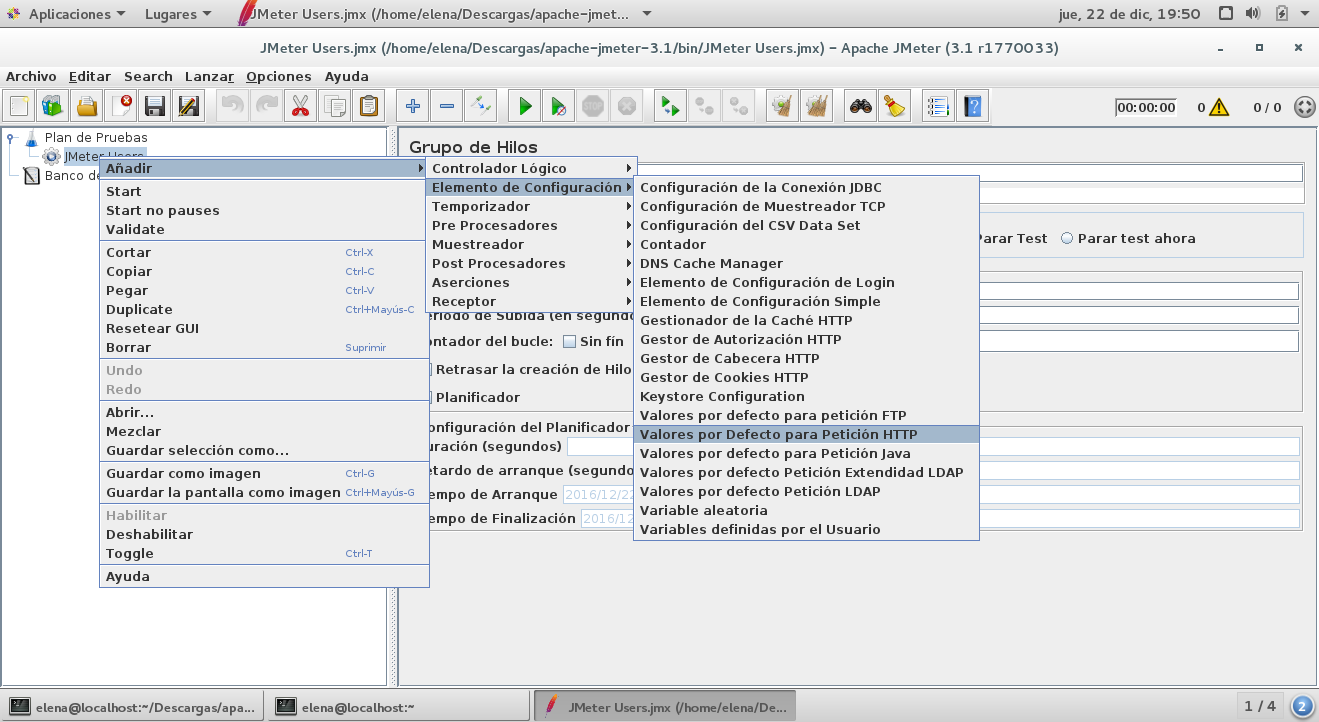
\includegraphics[width=14.7cm]{./img/ejercicio4_4.png} 	
	\caption{CentOS, JMeter - añadir valores de las peticiones HTTP por defecto.} \label{fig:ejercicio4_4}
\end{figure}

\begin{figure}[H] 
	\centering
	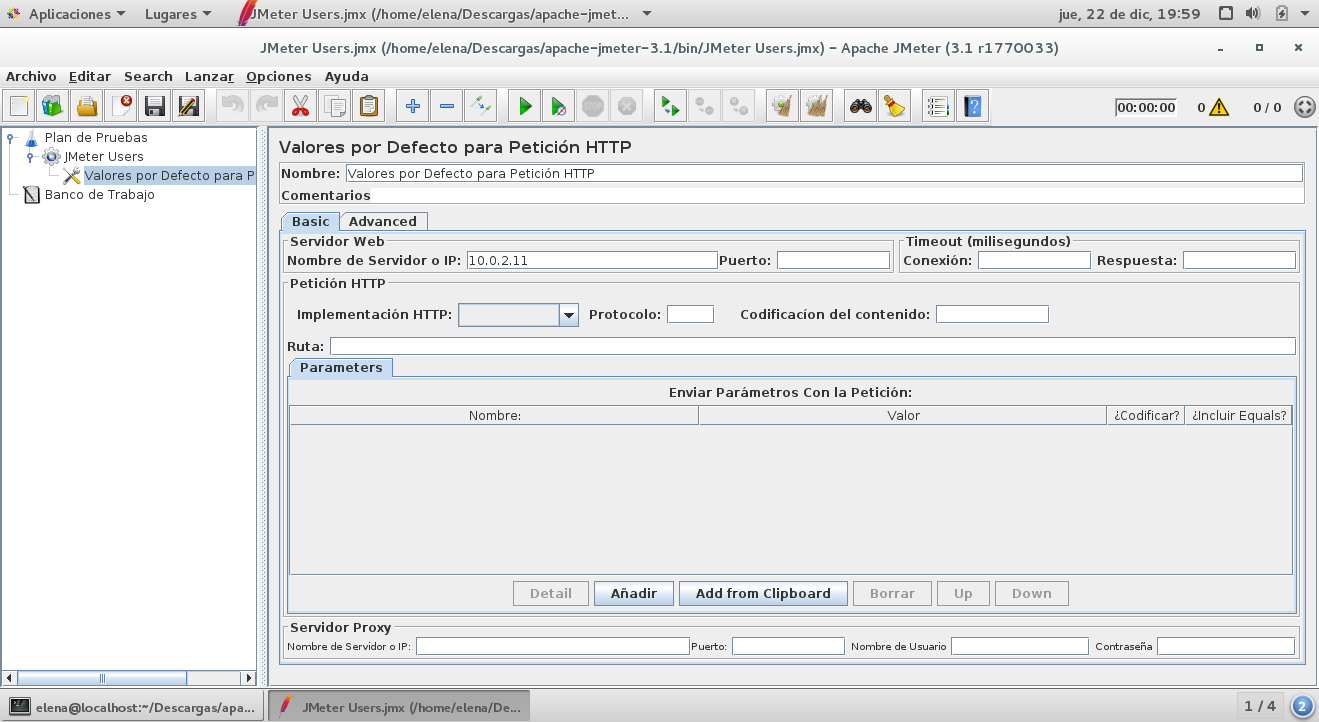
\includegraphics[width=14.7cm]{./img/ejercicio4_5.png} 	
	\caption{CentOS, JMeter - valores de las peticiones HTTP por defecto.} \label{fig:ejercicio4_5}
\end{figure}

\begin{figure}[H] 
	\centering
	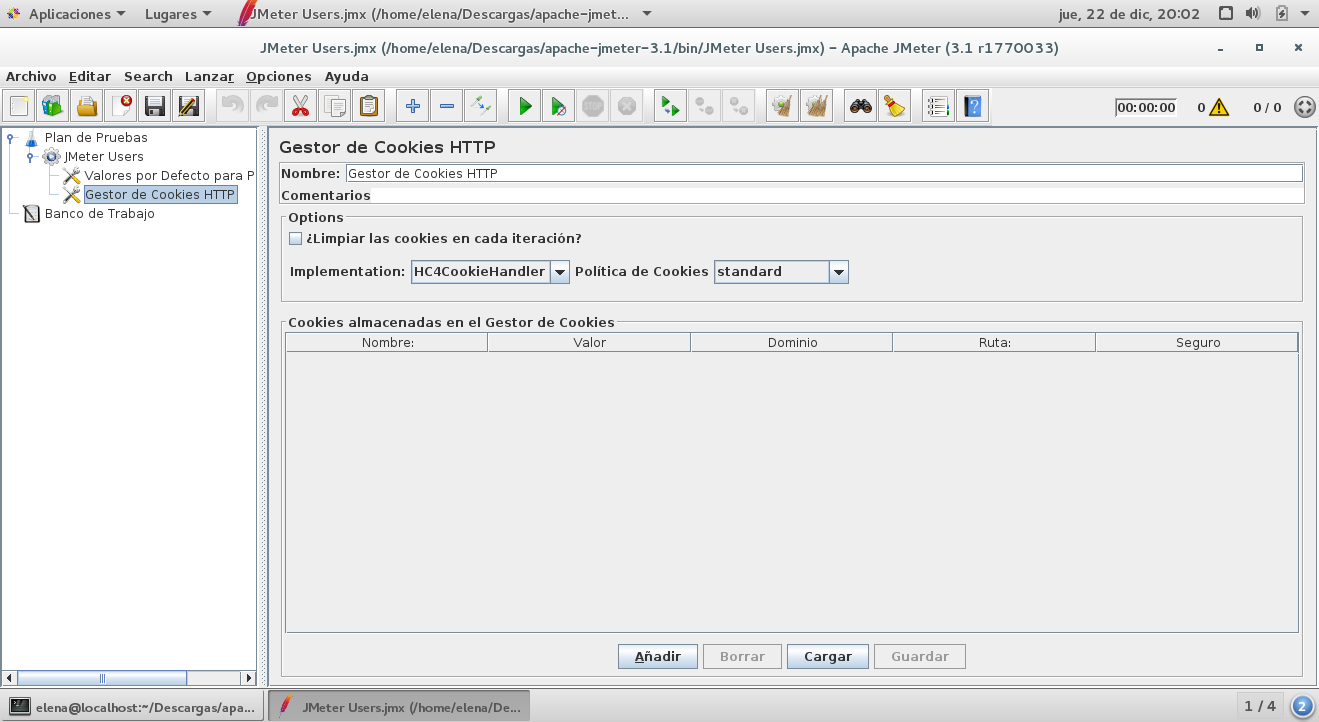
\includegraphics[width=14.7cm]{./img/ejercicio4_6.png} 	
	\caption{CentOS, JMeter - gestor de Cookies de HTTP.} \label{fig:ejercicio4_6}
\end{figure}

\begin{figure}[H] 
	\centering
	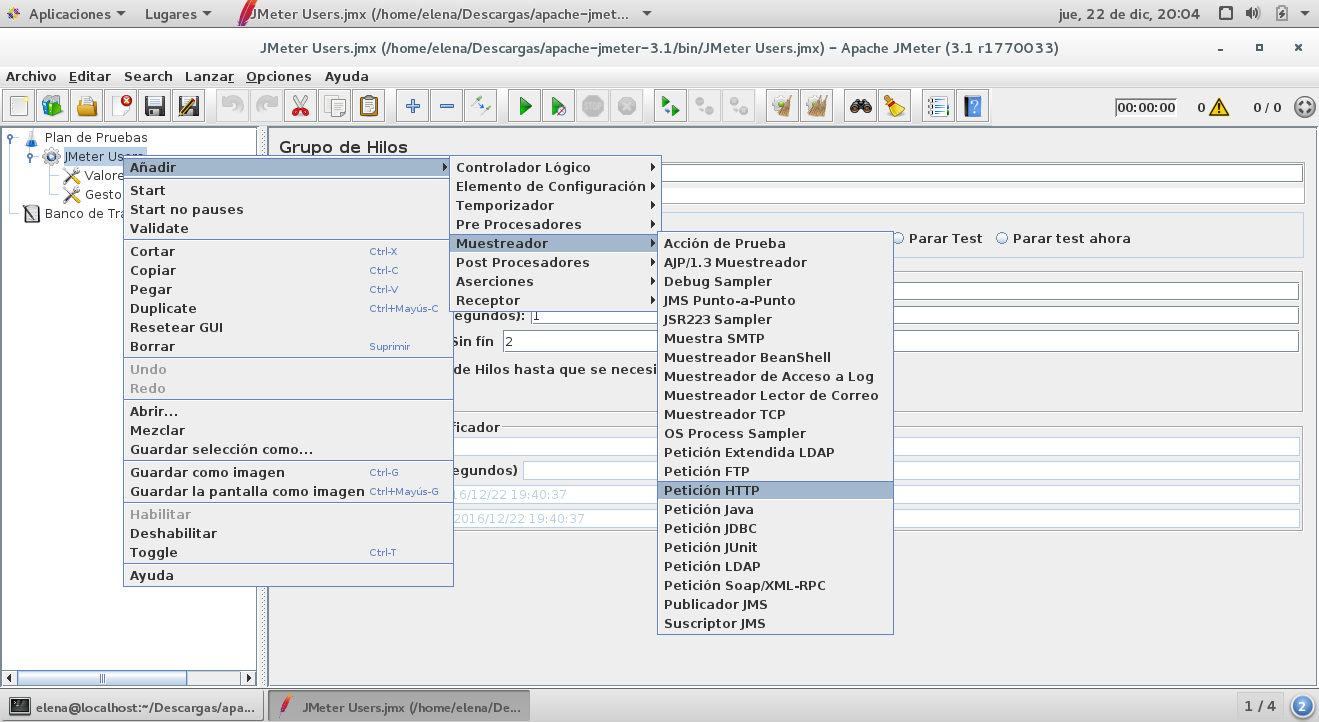
\includegraphics[width=14.7cm]{./img/ejercicio4_7.png} 	
	\caption{CentOS, JMeter - añadir peticiones HTTP.} \label{fig:ejercicio4_7}
\end{figure}

\begin{figure}[H] 
	\centering
	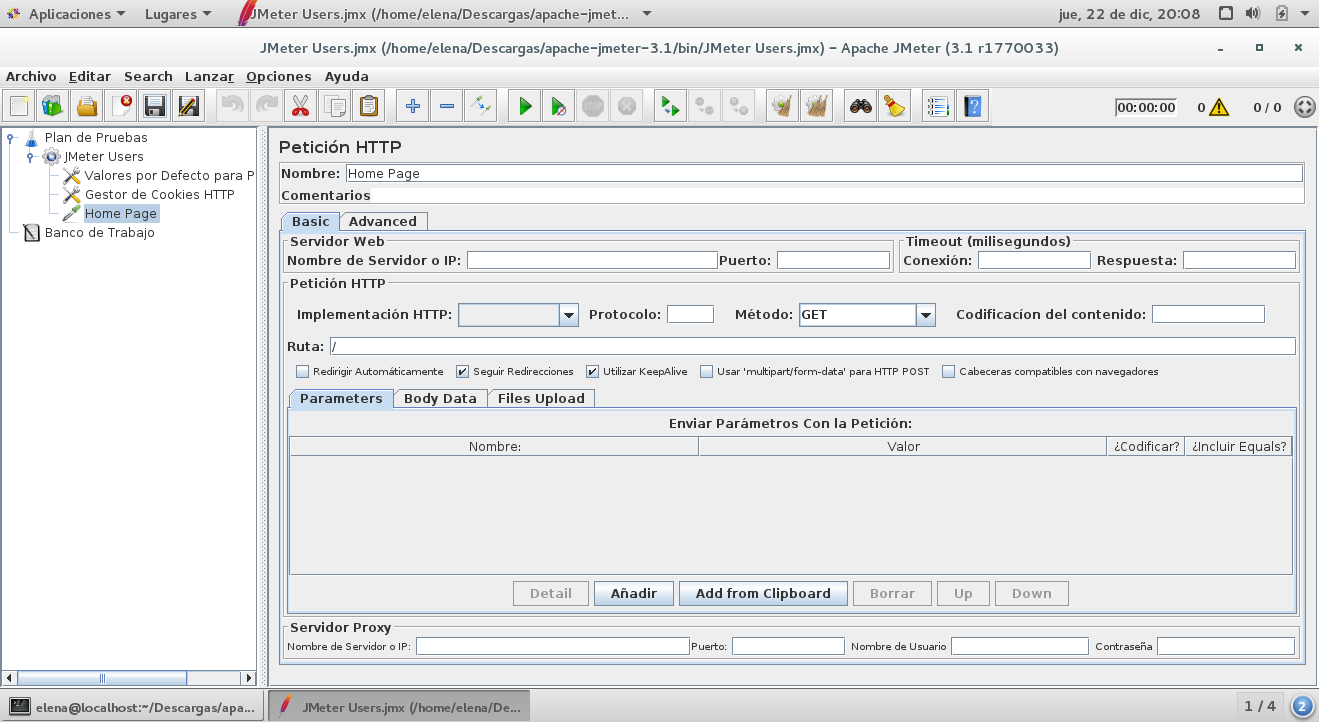
\includegraphics[width=14.7cm]{./img/ejercicio4_8.png} 	
	\caption{CentOS, JMeter - peticiones HTTP.} \label{fig:ejercicio4_8}
\end{figure}

\begin{figure}[H] 
	\centering
	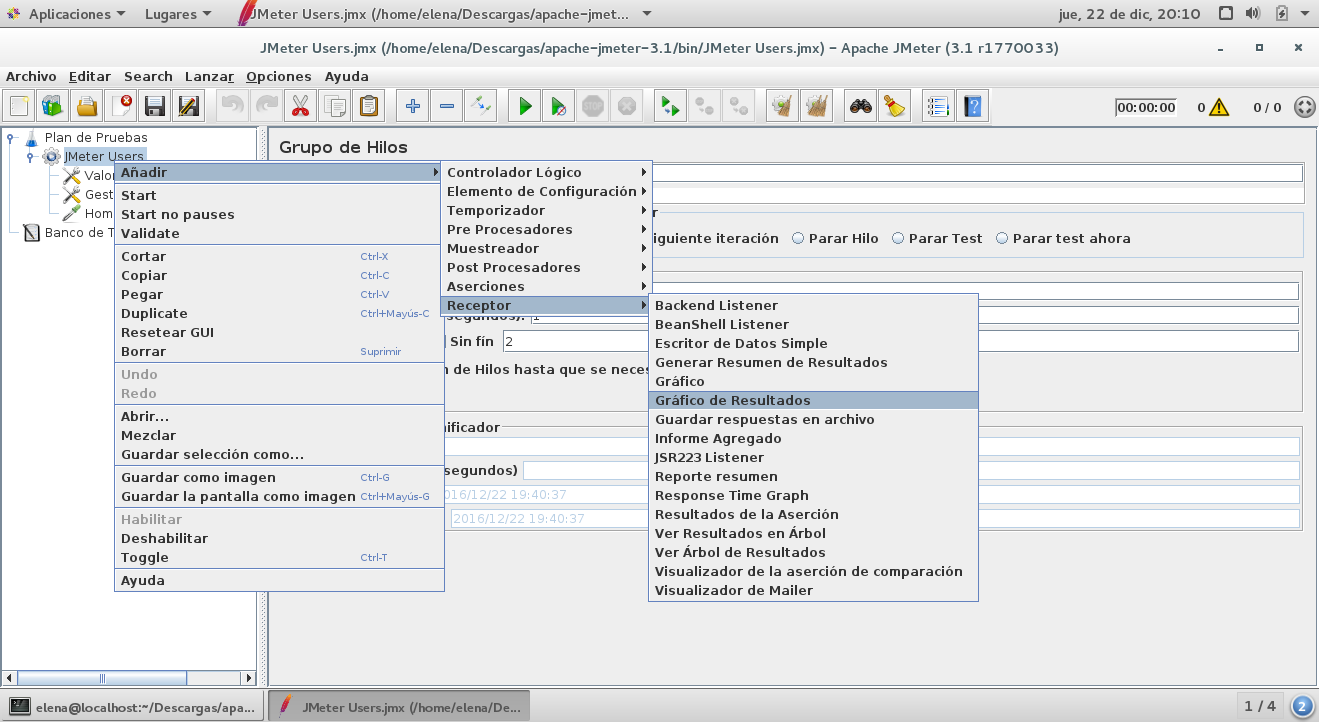
\includegraphics[width=14.7cm]{./img/ejercicio4_9.png} 	
	\caption{CentOS, JMeter - añadir gráfico.} \label{fig:ejercicio4_9}
\end{figure}

\begin{figure}[H] 
	\centering
	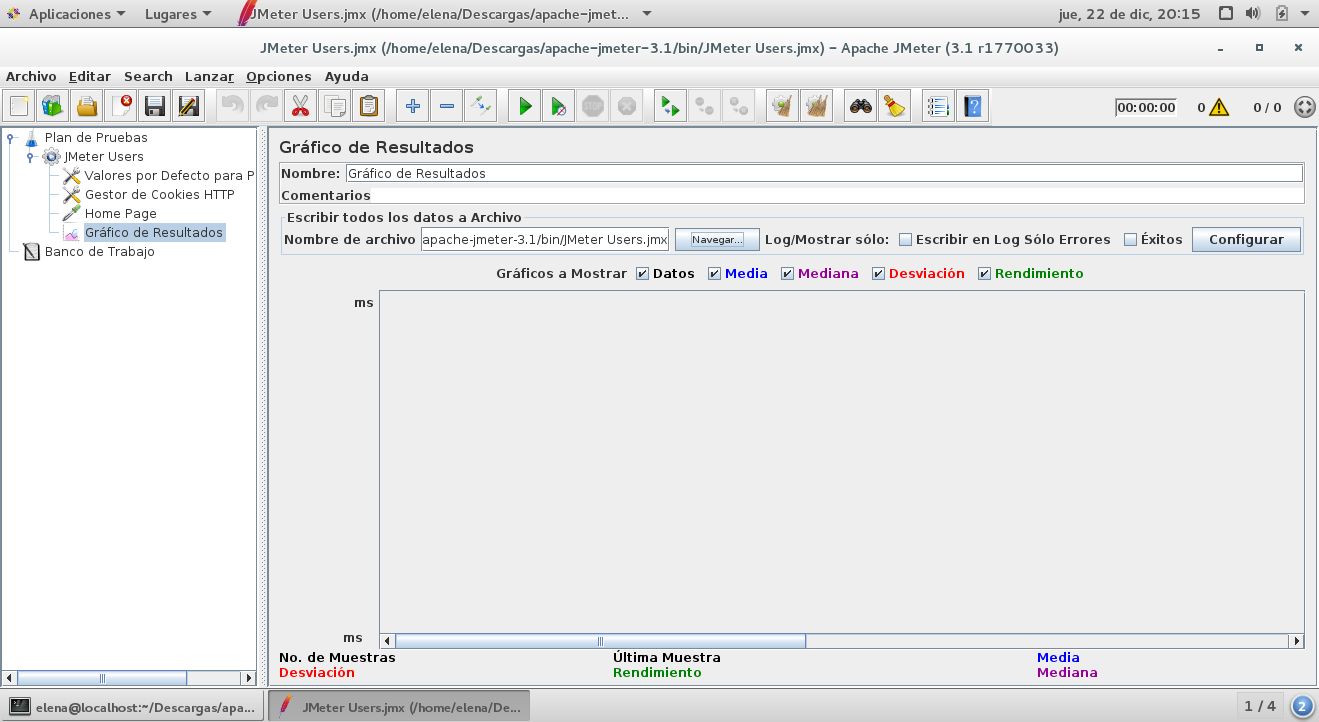
\includegraphics[width=14.7cm]{./img/ejercicio4_10.png} 	
	\caption{CentOS, JMeter - gráfico de resultados.} \label{fig:ejercicio4_10}
\end{figure}

\begin{figure}[H] 
	\centering
	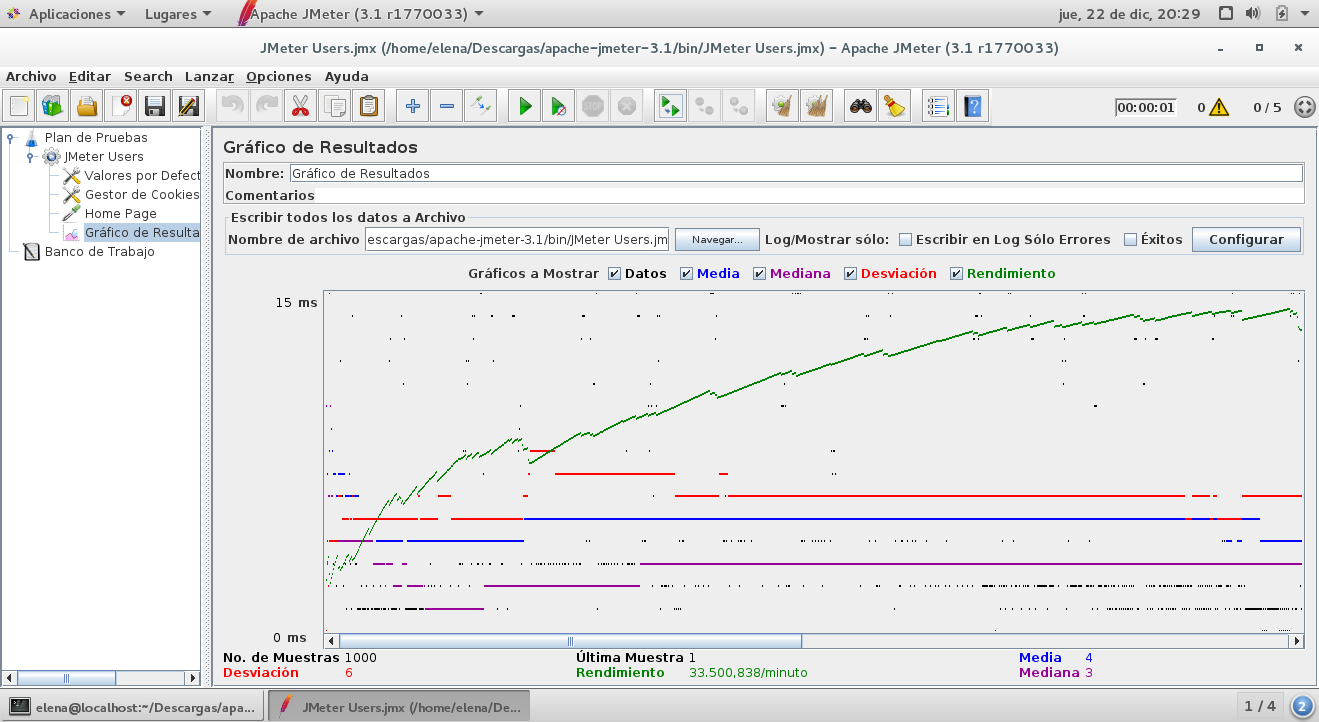
\includegraphics[width=14.7cm]{./img/ejercicio4_11.png} 	
	\caption{CentOS, JMeter - gráfico de resultados hacia Ubuntu Server.} \label{fig:ejercicio4_11}
\end{figure}

\begin{figure}[H] 
	\centering
	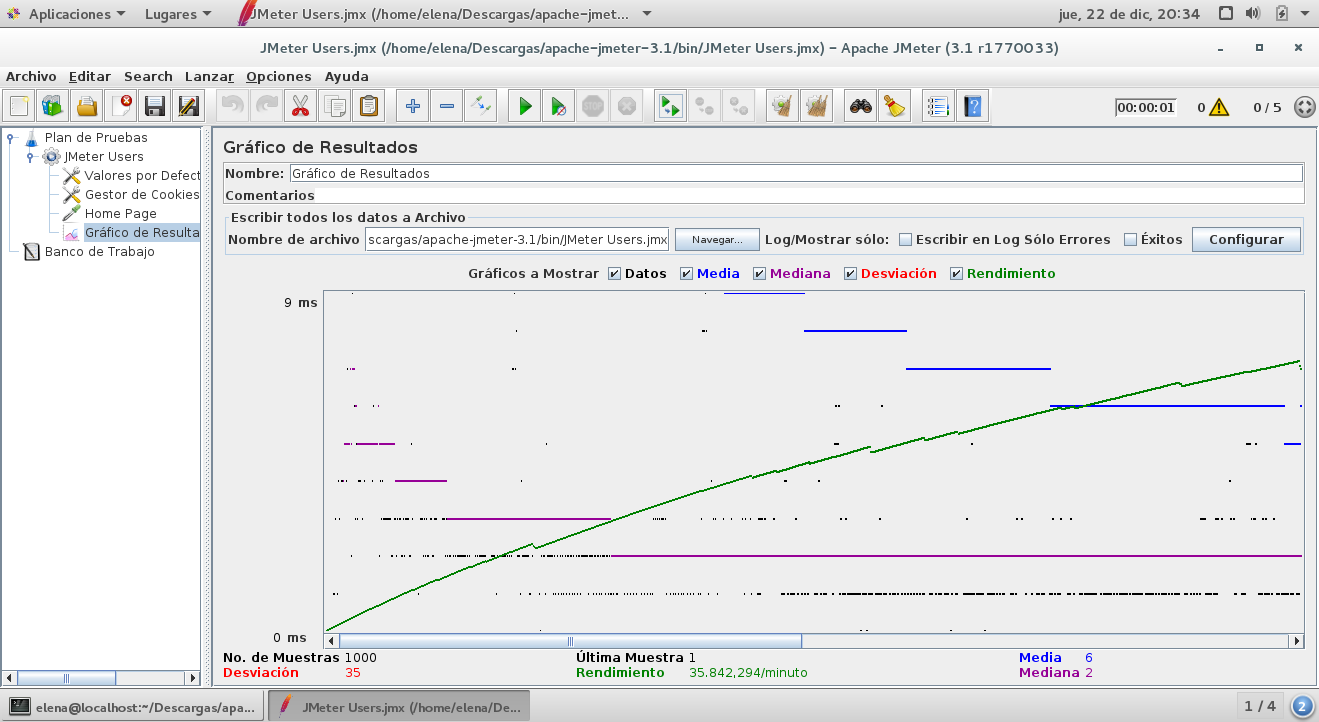
\includegraphics[width=14.7cm]{./img/ejercicio4_12.png} 	
	\caption{CentOS, JMeter - gráfico de resultados hacia Windows.} \label{fig:ejercicio4_12}
\end{figure}

\begin{figure}[H] 
	\centering
	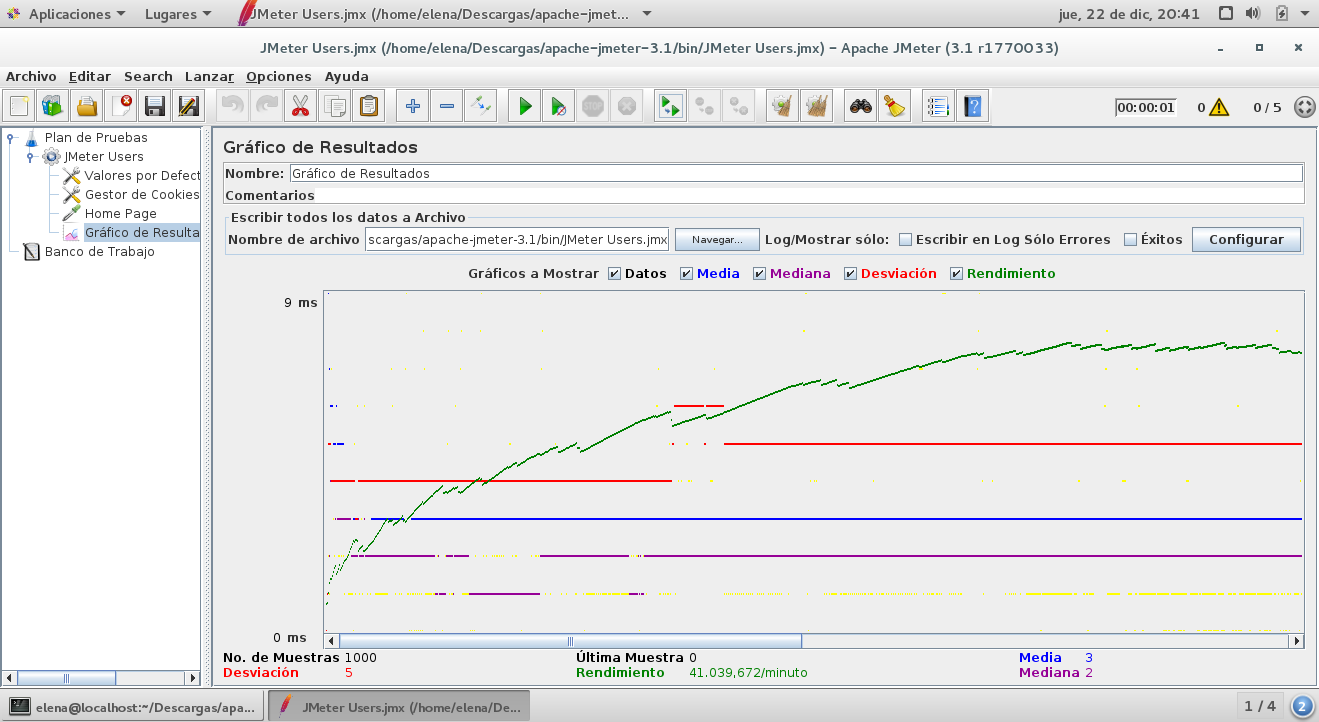
\includegraphics[width=14.7cm]{./img/ejercicio4_13.png} 	
	\caption{CentOS, JMeter - gráfico de resultados hacia CentOS.} \label{fig:ejercicio4_13}
\end{figure}



%----------------------------------------------------------------------------------------
%	Cuestión 5
%----------------------------------------------------------------------------------------

\section{Cuestión 5:}
\subsection{Programe un benchmark usando el lenguaje que desee. El benchmark debe incluir:}

\begin{enumerate}
	\item \textbf{Objetivo del benchmark.}
	\item \textbf{Métricas (unidades, variables, puntuaciones, etc.).}
	\item \textbf{Instrucciones para su uso.}
	\item \textbf{Ejemplo de uso analizando los resultados.}
\end{enumerate}

\textbf{Tenga en cuenta que puede comparar varios gestores de BD, lenguajes de programación web (tiempos de ejecución, gestión de memoria, ...), duración de la batería, servidor DNS, etc. . Alternativamente, puede descargar alguno de algún repositorio en github y modificarlo según sus necesidades.}\\

\subsubsection{Objetivo del benchmark.} 
Voy a utilizar como base un ejercicio que realizamos en la asignatura de Arquitectura de Computadores el cual calcula el tiempo de ejecutar n operaciones en coma flotante de forma secuencial. El benchmark está escrito en C y realiza un número de operaciones de suma, multiplicación y división. El código del benchmark está incluido en el zip con nombre ``benchmark\_float.c''\\

Por lo tanto el objetivo del benchmark es analizar el tiempo que tarda el procesador en realizar operaciones en coma flotante. Mostrará el tiempo de forma independiente de las sumas, multiplicaciones y divisiones.


\subsubsection{Métricas (unidades, variables, puntuaciones, etc.).}
Como ya hemos dicho anteriormente el benchmark realiza una medición del tiempo de ejecución, por cada una de las operaciones, la cual se muestra en segundos.

\subsubsection{Instrucciones para su uso.}
Para compilar el benchmark se usará la siguiente línea (lrt es una librería de tiempo real): 
\texttt{sudo gcc benchmark\_float.c -o benchmark\_float –lrt}\\

Para ejecutarlo se usa: \texttt{./benchmark\_float <longitud>}, siendo ``longitud'' un valor pasado como parámetro por el que dependerá el número de operaciones realizadas, siendo su valor máximo 1000, por lo que si se introduce un valor superior a éste se limita a 1000.


\subsubsection{Ejemplo de uso analizando los resultados.}

Los resultados de las ejecuciones del benchmark se pueden ver en las figuras: Ubuntu anfitrión \ref{fig:ejercicio5_1}, CentOS \ref{fig:ejercicio5_2} 

\begin{figure}[H] 
	\centering
	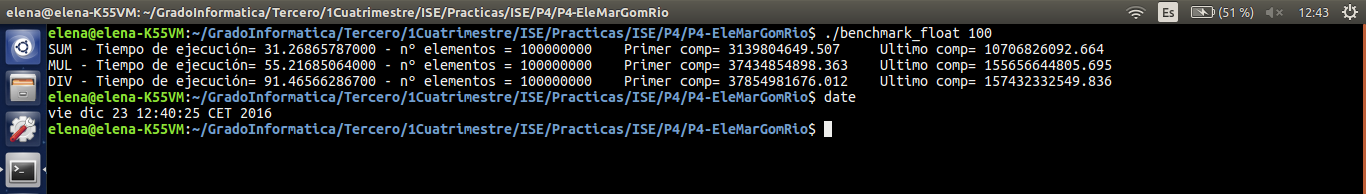
\includegraphics[width=14.7cm]{./img/ejercicio5_1.png} 	
	\caption{Ubuntu anfitrión, resultados del benchmark.} \label{fig:ejercicio5_1}
\end{figure}

\begin{figure}[H] 
	\centering
	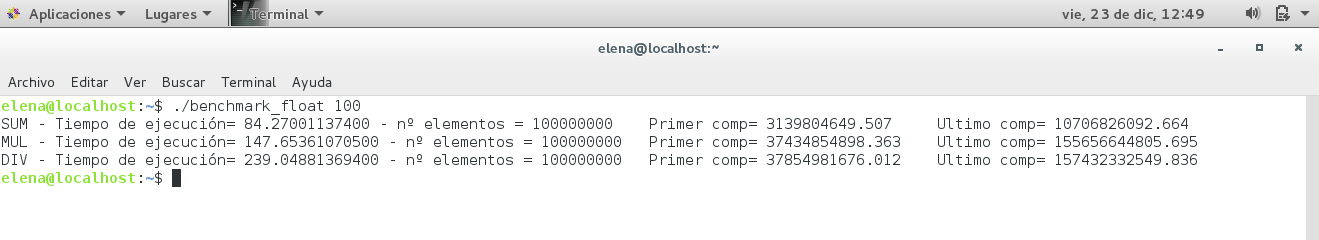
\includegraphics[width=14.7cm]{./img/ejercicio5_2.png} 	
	\caption{CentOS, resultados del benchmark.} \label{fig:ejercicio5_2}
\end{figure}


Para poder comparar mejor los tiempos del benchmark extraigo los tiempos en la tabla \ref{comparativa_bench} que se muestra a continuación.

\begin{table}[H]
\centering
\small
\setlength\tabcolsep{2pt}
\caption{Tiempos de la ejecución del benchmark.}
\label{comparativa_bench}
\begin{tabular}{|c|c|c|c|}
\hline
\textbf{SO}      & \textbf{Suma (s)} & \textbf{Multiplicación (s)} & \textbf{División (s)}  \\ \hline
\textbf{CentOS}  & 84.27          & 147.65             & 239.05 \\ \hline
\textbf{Ubuntu}  & 31.27         & 55.22          & 91.47                  \\ \hline
\end{tabular}
\end{table}

Se puede observar claramente que el anfitrión con Ubuntu es mucho mejor que CentOS en este tipo de operaciones.


%------------------------------------------------

\bibliography{citas} %archivo citas.bib que contiene las entradas 
\bibliographystyle{plain} % hay varias formas de citar

\end{document}
